\documentclass[conference]{IEEEtran}
\IEEEoverridecommandlockouts
% The preceding line is only needed to identify funding in the first footnote. If that is unneeded, please comment it out.
\usepackage{cite}
\usepackage{authblk}
\usepackage{amsmath,amssymb,amsfonts}
\usepackage{algorithmic}
\usepackage{graphicx}
\usepackage{textcomp}
\usepackage{xcolor}
\def\BibTeX{{\rm B\kern-.05em{\sc i\kern-.025em b}\kern-.08em
    T\kern-.1667em\lower.7ex\hbox{E}\kern-.125emX}}
\begin{document}

\title{A Survey of Security Threats in Federated Laearning}

\author[1]{Yunhao Feng}
\author[1]{Yinjian Hou}
\author[1]{Yanming Guo}
\affil[1]{National University of Defense Technology}

\maketitle

\begin{abstract}
    Federated learning is a distributed machine learning paradigm that emerged as a solution to the need for privacy protection in artificial intelligence. 
    Federated learning, like traditional machine learning, is threatened by backdoor attacks, Byzantine attacks, and adversarial attacks. 
    This weakness is exacerbated by the inaccessibility of data in federated learning, 
    which makes it more difficult to defend against these threats.
    This points to the need for further research into defensive approaches to make federated learning a real solution for distributed machine learning paradigm with securing data privacy.
    In this article, we provide an extensive survey of the threats to federal learning, 
    and their countermeasures accordingly. 
    This survey provides a taxonomy of these threats and their defense methods, 
    describing the general situation of this vulnerability in federal learning and how to overcome it. 
    We also sort out the relationship between these methods, their advantages and disadvantages, and put forward the future research directions.
\end{abstract}



\section{Introduction}
Artificial intelligence (AI) can analyze large amounts of data, 
identify patterns, make decisions, improve efficiency, and solve complex problems 
in various fields.
Nevertheless, most existing AI techniques rely on rich and high-quality 
datasets to train a highly accurate machine learning model.
For example, while training the SAM model, 
FACEBOOK \cite{b1}  built the largest segmented dataset ever, 
building more than 1 billion masks on 11 million images.

However, a more practical reality is that most companies cannot 
construct such large and high-quality datasets like Facebook 
when training their model. 
Insufficient samples and low data quality are the actual challenges 
that most companies face in model training. 
To address this problem, one possible solution 
is the sharing of data among multiple organizations or companies. 
However, this approach presents several new challenges.

The first challenge relates to data privacy. 
The data held by organizations may contain sensitive information, 
such as medical or financial data of their users. 
Additionally, new legal frameworks are increasingly 
emphasizing the protection of individual data privacy \cite{b2}. 
Privacy protection introduces restrictions that prevent 
privacy data from leaving its originating organization 
and being uploaded to central server.
The second challenge is related to the diverse organizations of data. 
Data from different organizations provides an increase in available data, 
driving advancements in artificial intelligence models. 
However, due to the various organizations, 
storing and processing data from different organizations, 
as well as reducing communication costs between these organizations 
have become new challenge to overcome.

In response to such challenges, Google \cite{b3} developed a distributed 
machine learning framework called federated learning (FL). 
This framework allows each client 
to collectively train models without sharing their data.
In federated learning, the data of each client remains private and inaccessible 
to others. 
As shown in Fig.\ref{fig1}, in a typical federated learning framework, 
the server firstly sends a global model to all selected clients as local models. 
These clients then use their local datasets to train the 
local models and upload their trained model updates to the central server.
After receiving the updates from all selected clients, 
the server updates the global model by averaging the uploaded updates.
Finally, the server sends the updated global model to the selected clients. 
Throughout the training process, only the data owners 
have access to their local data. 
This approach ensures the protection of data 
from unauthorized access by other clients or the central server, 
while also reducing communication costs between the clients and the server. 
Federated learning can also improve the training speed and the performance of the
shared model while protecting privacy of the participants' training datasets\cite{b4}.


\begin{figure}[htbp]
    \centerline{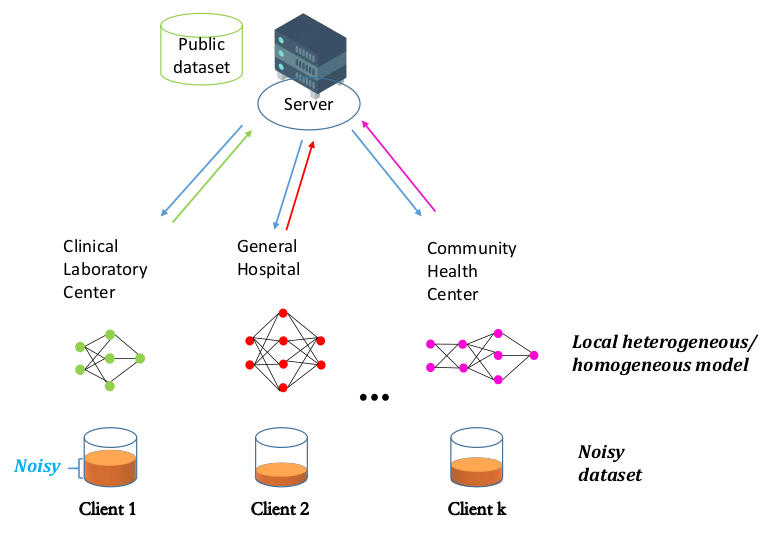
\includegraphics[width=0.8\linewidth,height=0.6\linewidth]{picture/f1.png}}
    \caption{The server firstly sends a global model to all selected clients as local models. 
    These clients then use their local datasets to train the 
    local models and upload their trained model updates to the central server.
    After receiving the updates from all selected clients, 
    the server updates the global model by averaging the uploaded updates. 
    Throughout the training process, only the data owners 
    have access to their local data. Finally, the server sends the updated global model to the selected clients.}
    \label{fig1}
\end{figure}


Due to the clear advantages of FL, 
FL has been applied to many fields in recent years, 
including computer vision\cite{b5,b6}, natural language processing\cite{b7,b8}, 
graph data analysis\cite{b9,b10}, and more.
However, further research has shown that federated learning 
also faces numerous security risks, 
such as backdoor attacks, adversarial attacks, and Byzantine attacks. 
The distributed nature of federated learning clients 
makes it more challenging to guarantee 
the trustworthiness of each client. 
Consequently, compared to traditional centralized machine learning, 
federated learning is more susceptible to attacks.

We primarily enumerates backdoor attacks, adversarial attacks, 
and Byzantine attacks in federated learning, 
along with their corresponding defense methods. 
These attacks pose significant threats to federated learning systems, 
and in response to these new threats, several FL defense methods have been proposed.

However, existing defense methods are predominantly attack-driven, 
meaning they can only defend against known attack techniques, 
while acknowledging that adversaries aware of these defenses can bypass them. 
Since defense methods are primarily developed based on observations 
and assumptions rather than thorough understanding of attack methods 
and learning algorithms, 
a comprehensive and in-depth survey is required to gain a better understanding of 
threats and defenses in FL.

In previous studies\cite{b11,b12,b13,b14,b15}, 
researchers have explored some attacks and defense strategies in the context 
of federated learning. 
However, these studies often categorize backdoor attacks 
and Byzantine attacks as data poisoning attacks and 
rarely delve into adversarial attacks in the field of federated learning. 
We believe that simply classifying backdoor attacks and Byzantine attacks 
as data poisoning attacks is insufficient 
because their attack methods are not limited to just data poisoning.
In this paper, we propose a new classification approach for these two 
types of attacks and provide an overview of their corresponding defense mechanisms. 
Addressing the lack of content on adversarial attacks in previous surveys, 
we supplement this paper with content on adversarial attacks and their defense 
mechanisms. 
Furthermore, we conduct a detailed analysis of the effectiveness and limitations 
of these attack methods and their corresponding defense mechanisms. 
The aim of this paper is to enhance understanding of the threats faced 
by federated learning and their defense mechanisms, 
and to assist the academic and industrial communities in 
developing more robust federated learning systems. 
To this end, we also discuss future research directions 
regarding the security issues of federated learning from multiple perspectives.

\section{Threat Model}
\begin{figure}[htbp]
    \centerline{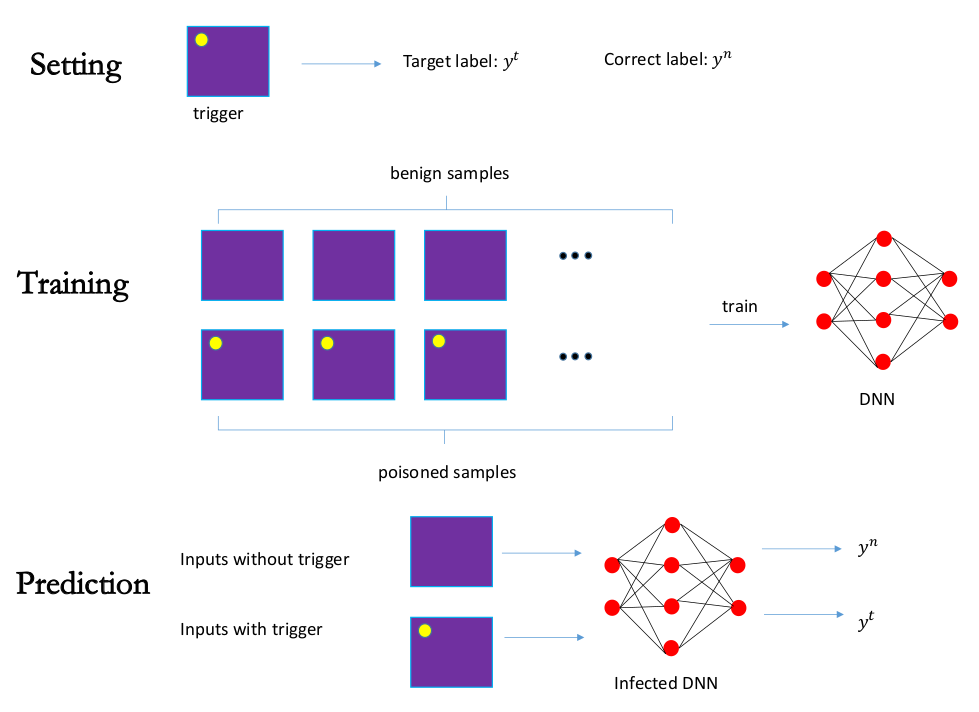
\includegraphics[width=0.8\linewidth,height=0.6\linewidth]{picture/backdoor_attack.png}}
    \caption{Backdoor attacks refer to a malicious backdoor 
    added to the global model by malicious participants during training process. 
    The backdoor can be triggered by specific inputs, 
    allowing attackers to control the outputs of the model. 
    The goal of the backdoor attacks is to make the model maintain the normal 
    outputs on the normal samples, but the outputs expected by attackers are 
    shown in the backdoor samples.}
    \label{fig2}
\end{figure}

In this section, we give a preliminary introduction to the definitions of the three attacks discussed in this paper.
As shown in Fig.\ref{fig2}, backdoor attacks\cite{b16,b17,b18,b19,b20} refer to a malicious backdoor 
added to the global model by malicious participants during training process. 
The backdoor can be triggered by specific inputs, 
allowing attackers to control the outputs of the model. 
The goal of the backdoor attacks is to make the model maintain the normal 
outputs on the normal samples, but the outputs expected by attackers are 
shown in the backdoor samples.

\begin{figure}[htbp]
    \centerline{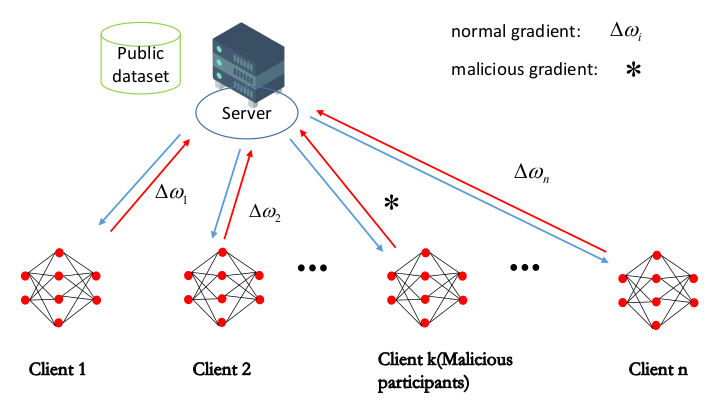
\includegraphics[width=0.8\linewidth,height=0.6\linewidth]{picture/byattack.png}}
    \caption{In Byzantine attacks, there exist one or more malicious participants 
    in the federated learning system 
    who disrupt the training process by sending incorrect or misleading updates 
    to the central server, causing abnormal convergence}
    \label{fig3}
\end{figure}

The meaning of Byzantine attacks\cite{b21,b22,b27} is that 
there exist one or more malicious participants in the federated learning system 
who disrupt the training process by sending incorrect or misleading updates 
to the central server, causing abnormal convergence, as shown in Fig.\ref{fig3}.

\begin{figure}[htbp]
    \centerline{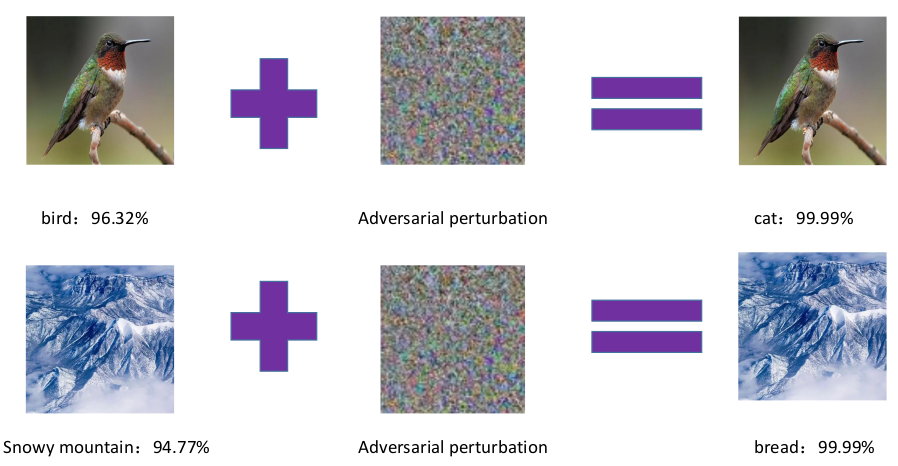
\includegraphics[width=0.8\linewidth,height=0.6\linewidth]{picture/adversarial_attack.png}}
    \caption{Adversarial attacks require adding subtle and 
    carefully crafted perturbations 
    to the input data to deceive the model and 
    cause it to make incorrect predictions. }
    \label{fig4}
\end{figure}

As shown in Fig.\ref{fig4}, adversarial attacks\cite{b23,b24,b25,b26} require adding subtle and carefully crafted perturbations 
to the input data to deceive the model and cause it to make incorrect predictions. 
These attacks pose significant challenges in designing and implementing 
federated learning systems. 
For instance, personalized advertising recommendation systems 
are often classic examples of federated learning systems 
and malicious participants can exploit backdoors embedded in the global model 
to increase the quantity and frequency of their own ad placements, 
gaining unfair advantages. 
Therefore, it is crucial to address these robustness or security issues 
in federated learning.

Naturally, defense methods have been proposed and applied in federated learning 
to mitigate these threats. 
For example, knowledge distillation\cite{b28} and knowledge erasure\cite{b29} 
are commonly used to counteract backdoor attacks. 
Adversarial training\cite{b23,b24} has been introduced as a measure to tackle 
the threat of adversarial attacks.

Prior to delving into the details of the threats of federated
learning, it is essential to make classifications of these threats. 
Specifically, we can categorize these threats into two main stages: the
training phase and the inference phase. Additionally, we
can also differentiate them between untargeted attacks and targeted
attacks based on whether a specific target is present or
not.  

\subsection{Training Phase and Inference Phase}
\subsubsection{Training Phase}
Attacks that occur during the model training process are
intended to either disrupt or impact the federated learning model itself. 
During the training stage, 
backdoor attacks involve the insertion of a backdoor into the model, whereas
input deception models with triggers are utilized during the
reasoning stage to cause the model to generate incorrect results\cite{b30},\cite{b31}.
Byzantine attacks disrupt the convergence of the model by utilizing malicious
clients or servers\cite{b21}.
\subsubsection{Inference Phase}Attacks that occur during the reasoning phase are
typically intended to alter the model's reasoning outcomes and deceive it
into generating incorrect outputs\cite{b47}. 
Adversarial attacks, leverage the model's vulnerability
to disturbances and utilize samples with adversarial perturbations as input
to the model, causing it to produce erroneous outcomes.

\subsection{Untargeted and Targeted}
\subsubsection{Untargeted attacks}Untargeted attacks are designed to compromise
the integrity of the target model in an arbitrary manner.
Byzantine attack is one form of untargeted attacks that involves
uploading malicious gradients to the server in an arbitrary manner,
with the goal of causing the global model to fail\cite{b48},\cite{b49},\cite{b50},\cite{b51}.
\subsubsection{Targeted Attacks}A targeted attack is executed with
the aim of inducing the model to produce the target label specified by the
adversary for specific testing examples, while keeping the testing error for
other testing examples unaffected\cite{b51}. Backdoor attack is a typical application of targeted attack.


\section{Backdoor Attack}
Backdoor attacks on deep neural networks require malicious backdoors to be secretly implanted in the model. 
This enables the model to function
normally when processing benign inputs, but triggers  pre-defined
malicious behavior when presented with a specific malicious trigger.
The first neural backdoor in centralized settings can be traced
back to 2013\cite{b52},\cite{b53}.

Due to the unique nature of federated learning, whereby the model is trained
on individual clients, it is more susceptible to backdoor attacks compared
to the general centralized training model. These types of attacks in federated
learning can be divided into two categories based on the different stages at
which the adversary inserts the backdoor into the training pipeline: data
poisoning attacks and model poisoning attacks.

\subsection{Data Poisoning Attack}
In data poisoning attacks, it is assumed that the adversary has full control
over the training data collection process of compromised clients. Then the poisoned
dataset typically consists of a combination of clean data with ground-truth labels
and data with backdoor triggers that have targeted labels.

\subsubsection{Visible Poisoning}
Early methods of  backdoor attacks in federated learning can rely on a single trigger,
meaning that all corrupted clients inject the same trigger into their local
training dataset. The triggers employed in this method are usually predetermined,
such as a square located at redundant pixels in the image. During reasoning,
the inserted trigger is used on a malicious client to activate the aggregation model\cite{b24},\cite{b27}.
While the effectiveness of inserting the backdoor has been shown to be significant,
the aforementioned approach merely transfers backdoor attacks from centralized
learning directly to federated learning, without fully leveraging
the distributed nature of the latter. This is
because the same trigger is embedded in all adversarial clients.

So some studies take advantage of the characteristics of federated learning to carry out backdoor attacks.
As shown in Fig.\ref{fig8}, Xie et al. \cite{b59} proposed a distributed backdoor attack (DBA) that decomposes a global trigger 
pattern, similar to a centralized attack, into local patterns and embeds
them into different malicious clients. Compared to traditional methods that insert
the same trigger, DBA is more efficient and covert due to its hidden local
trigger mode, making it easier to bypass robust aggregation rules.

\begin{figure}[htbp]
    \centerline{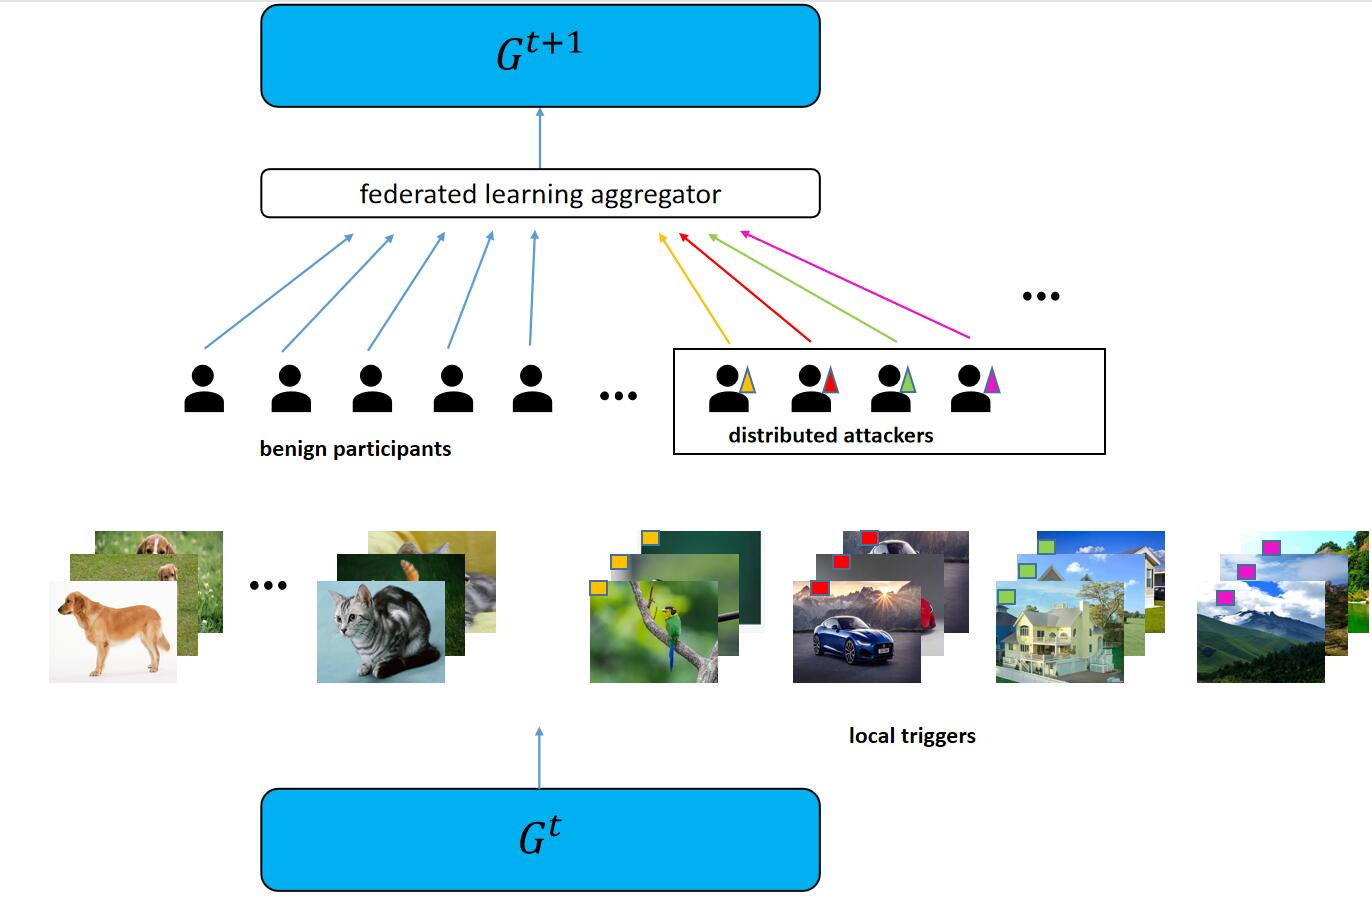
\includegraphics[width=0.8\linewidth,height=0.6\linewidth]{picture/f8.jpg}}
    \caption{DBA decomposes a global trigger 
    pattern, similar to a trigger in centralized attack, into local patterns and embeds
    them into different malicious clients.}
    \label{fig8}
\end{figure}

But distributed backdoors are also easy to detect, and if the static triggers are changed to dynamic, 
the backdoors will be more difficult to detect.
Salem et al \cite{b60} conducted a
clear and systematic study on the feasibility of dynamic flip-flops,
which can facilitate the backdoor attacks by generating antagonistic
network algorithms to create triggers. This way, the same tags can be
hijacked with different trigger patterns that share similar potential
representations and positions. Li et al \cite{b61} also conducted a direct
investigation of dynamic triggers.

These triggers can be flexibly produced
during the attack phase, as they maintain their effectiveness even
under substantial changes. The results of the study show that dynamically
triggered backdoor attacks are more powerful, and they require new techniques
to be defeated because they break the static trigger hypothesis of most current
defense systems.

Despite the potential threat of data poisoning attacks in federated learning,
they face many practical limitations due to the unique distributed characteristics \cite{b251}.
This is because the data distribution and model aggregation steps in federated learning tend to neutralize
most of the contributions of the backdoor model, leading to rapid forgetting of the backdoor by the global model.
In light of this situation, Wang et al.\cite{b251} proposed selecting poisoning samples from edge data to reduce the
forgetting effection caused by model updating.

Dai et al.\cite{b64} proposed a new backdoor attack method called Chameleon,
which enables attackers to create more persistent visual backdoors by adapting
to peer-to-peer images. The durability of the backdoor largely depends
on the existence of two types of identical benign images that are closely
related to the toxic image: Interferers, which are images that share
the same original tag as the toxic image. And facilitators, which are
images with the target back tag. Interferers can cause update conflicts
between toxic updates and benign updates, which may reduce the accuracy of
the backdoor. Conversely, facilitators can help reintroduce backdoor
information into the federated learning model and mitigate the catastrophic
forgetting effect after the attacker leaves the training process. Inspired by
these observations, Chameleon is designed to amplify these effects and enhance
the durability of the backdoor.

\subsubsection{Invisible Poisoning}
In this context, the term 'invisible' denotes the user's ability to execute
a backdoor attack on a sample without requiring any additional actions to
be performed on the sample itself.


\begin{figure}[htbp]
    \centerline{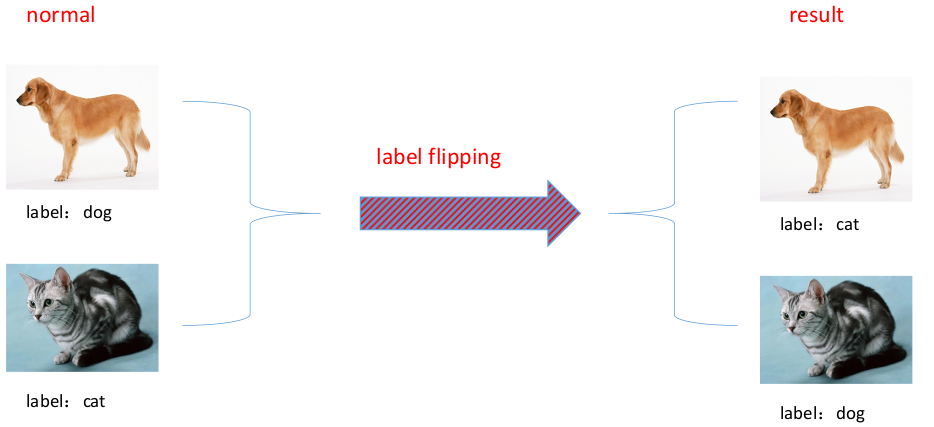
\includegraphics[width=0.8\linewidth,height=0.5\linewidth]{picture/f6.png}}
    \caption{Label Flipping.In this picture, some of the samples labeled 'dog' are flipped to 'cat' and the samples of 'cat'
    are flipped to 'dog'}
    \label{fig6}
\end{figure}

Label flipping is a widely recognized attack in centralized machine learning (ML),
as demonstrated in previous research studies\cite{b54},\cite{b55}. In addition,
it is also a suitable method for the federated learning (FL) scenario,
given its adversarial goal and capabilities\cite{b56}.
As shown in Fig.\ref{fig6}, some of the samples labeled 'dog' are flipped to 'cat' and the samples of 'cat'
are flipped to 'dog'.


Nevertheless, the label flipping technique has its limitations since it necessitates
modifying the label of the sample, making it less practical. 
Thus, an attack technique that is more covert and can deceive manual inspection would be more
appealing in this scenario.
As shown in Fig.\ref{fig7}, clean-label attack preserves the label of the poisoned data,
and the manipulated image still appears to be a benign sample\cite{b57},\cite{b58}. This type of attack
leverages feature collision, where the crafted poison examples continue to
resemble the source instances in visual appearance, while being closer to the
targeted instances in the latent feature space.

\begin{figure}[htbp]
    \centerline{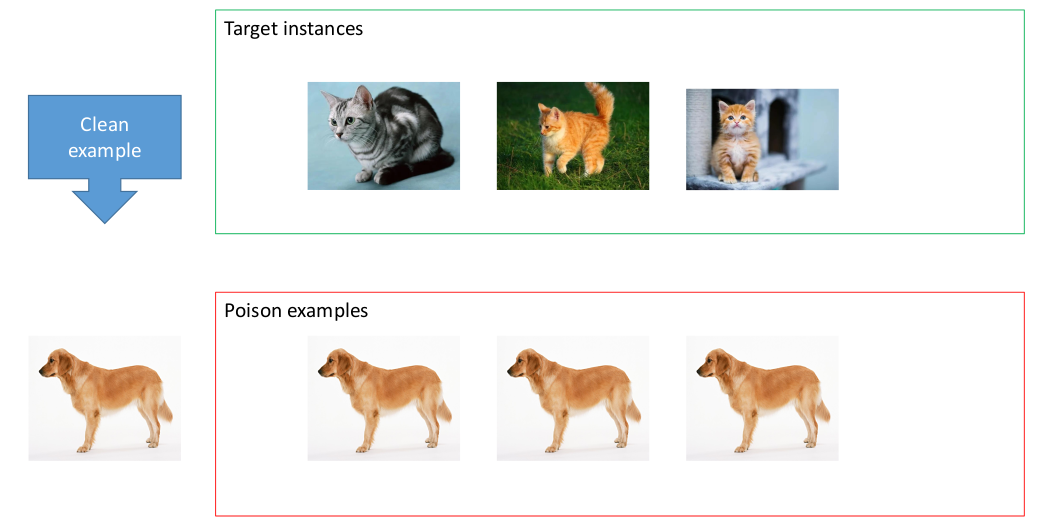
\includegraphics[width=0.8\linewidth,height=0.6\linewidth]{picture/f7.png}}
    \caption{Clean-label attack preserves the label of the poisoned data,
    and the manipulated image still appears to be a benign sample. This type of attack
    leverages feature collision, where the crafted poison examples continue to
    resemble the source instances in visual appearance, while being closer to the
    targeted instances in the latent feature space.}
    \label{fig7}
\end{figure}

Data poisoning faces the risks of being easily detected and traced. 
At the same time, the initial assumption that the attacker has complete control over the data set is difficult to achieve in many scenarios.


\subsection{Model Poisoning Attack}
To address the limitations of data poisoning attacks, we can not only focus on
improving the data poisoning technology itself, but also explore the potential
of model poisoning techniques. Since the average method is the most widely-used
approach for aggregating local updates from clients, a simple way to amplify
the backdoor effect is to prioritize updates from adversarial clients over
those from benign clients.

Bagdasaryan et al.\cite{b241} proposed the first backdoor attack against federated learning.
Their approach involves training a backdoor model that closely resembles the global
model, which is then used to replace the latest global model.
To improve the effectiveness of this replacement, they slow down
the learning rate to extend the lifespan of the backdoor model, and add an
anomaly detection term to the loss function to avoid detection. This
strategy requires careful evaluation of the global parameters and performs
better when the global model is close to convergence.

But similar to data poisoning, such direct substitutions are easily detected.
In order to avoid such substitutions,
Zhou et al.\cite{b63} proposed an optimization-based model poisoning attack that
involves injecting adversarial neurons into the redundant space of a neural network
to maintain the attack's concealment and persistence. To identify the redundant
space, the Hessian matrix is used to measure the update distance and direction of each neuron's main task.
An additional term is then added to the loss function to prevent poisoned neurons from being injected
in locations that are particularly relevant to the main task.
In a similar vein, Zhang et al.\cite{b62}
proposed a persistent backdoor attack called Neurotoxin. This method
relies on the empirical observation that the norm of a stochastic gradient
is primarily concentrated in a small number of 'heavy hitter' coordinates.
Neurotoxin identifies these heavy hitters using the top-k heuristic and
avoids them. By avoiding directions that are most likely to receive large
updates from benign devices, the chance of the backdoor being erased is mitigated.

Sun et al. \cite{b65}proposed a distance-aware attack (ADA), which enhances poisoning attacks
by identifying optimized target classes in the feature space. They addressed the challenge of
limited prior knowledge of customer data that competitors may face. To overcome this problem,
ADA infers the pairwise distances between different categories in the potential feature space
from the shared model parameters using backward error analysis. They conducted an extensive
empirical evaluation of ADA by varying attack frequency in three different image classification
tasks. As a result, ADA successfully improved the attack performance by 1.8 times in the most
challenging cases with attack frequency of 0.01x.

\subsection{Summary Of Federated Backdoor Attack}
The primary challenges of backdoor attacks in federated learning are how
to leverage the distributed nature of this approach, evade detector checks,
and ensure the persistence of the backdoors during multiple rounds of update
iterations. We identify three research directions for federated backdoor
attacks: using multiple malicious clients to insert backdoor attacks,
combining generation technology with backdoor attacks to insert dynamic backdoors, and conducting
research on persistent backdoor attacks in federated learning.

\section{Defenses against Backdoor Attack}
To mitigate the problem of backdoor attacks in
federated learning, various defensive techniques have been proposed.
Given that we previously categorized backdoor attacks as data poisoning
attacks and model poisoning attacks, we will now discuss defensive strategies
for each of these attack types.

\subsection{Defense Against Data Poisoning}
The simplest approach is to filter out poisoned data samples,
which aims to remove the poisoned samples from the training datasets.
After the filtering process, only benign samples or purified poisoned
samples are used during the training process, thus eliminating the
creation of backdoors from the source.

Tran et al.\cite{b67} are the first to investigate methods for filtering out malicious
samples from the training sets. They demonstrated that poisoned samples tend to
leave detectable traces within the covariance range of the feature representation.
Exploiting this insight, it is possible to filter out poisoned samples from
the training sets. Zeng et al. \cite{b68} revealed that poisoned samples of
existing attacks had some high-frequency artifacts even if their trigger
patterns are invisible in the input space. Based on this observation,
they designed a simple yet effective filtering method based on those artifacts.
Similarly, Chen et al. \cite{b69}proposed a two-stage filtering approach.
As shown in Fig.\ref{fig9}, in the first stage, activation values of samples in each class are clustered
into two groups. And in the second stage, it is determined which clusters
correspond to poisoned samples.


\begin{figure}[htbp]
    \centerline{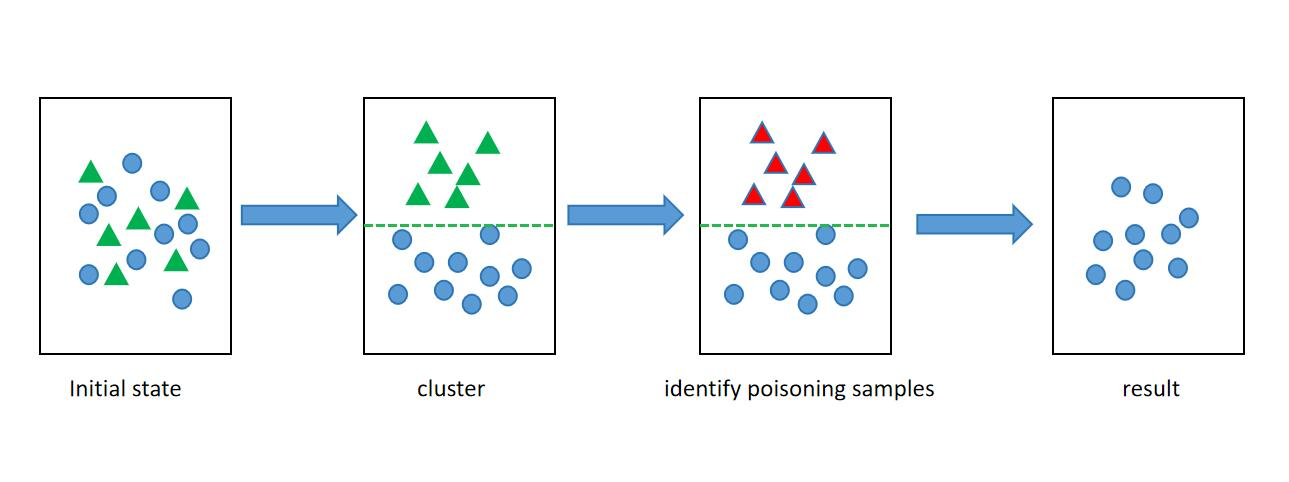
\includegraphics[width=0.8\linewidth,height=0.3\linewidth]{picture/two-stage-cluster.png}}
    \caption{In the first stage, activation values of samples in each class are clustered
    into two groups. And in the second stage, it is determined which clusters
    correspond to poisoned samples}
    \label{fig9}
\end{figure}


As is well known, backdoors are triggered during the inference stage.
Filtering out malicious samples from the testing samples during the inference stage can prevent the backdoor
from being activated. Gao et al. \cite{b71} proposed to filter attacked samples by overlaying various image patterns
on suspicious samples. The smaller the randomness of the input perturbation prediction, the higher the probability
that the suspicious sample is attacked. In \cite{b72}, Subedar et al. used model uncertainty to distinguish between
benign and attacked samples. Later, Du et al. \cite{b73} regarded filtering as outlier detection and proposed a
differential privacy-based filtering method. Recently, \cite{b74} proposed a lightweight method that can filter
attacked samples or prior hypotheses of trigger patterns without labeled samples.

However, Tang et al.\cite{b70} demonstrated that
simple target contamination can result in malicious and benign samples being
indistinguishable in the feature representation space. Therefore, most
sample filtering techniques are ineffective.

Based on data-driven defense methods, in addition to filtering out samples,
it is also possible to consider directly preprocessing the samples,
specifically by erasing any backdoors within them to prevent them from being embedded in the model.
Liu et al.\cite{b75} proposed a pre-trained autoencoder as a preprocessor to prevent malicious samples from embedding backdoors
by preprocessing the input samples without affecting data classification accuracy.

\begin{figure}[htbp]
    \centerline{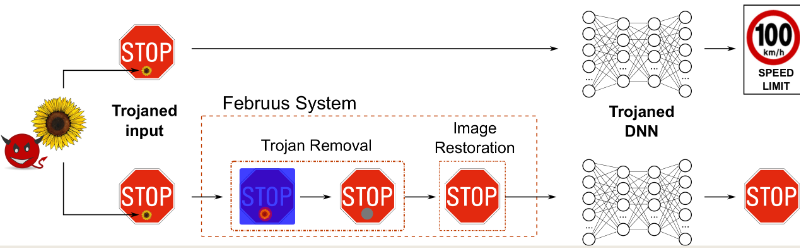
\includegraphics[width=1.0\linewidth,height=0.5\linewidth]{picture/f9.png}}
    \caption{Februus uses a GAN-based
    repair method to reconstruct the masked regions to mitigate their 
    adverse effects (such as benign accuracy reduction).}
    \label{fig10}
\end{figure}

Doan et al. \cite{b76} proposed a two-stage image processing method called Februus, in which,
in the first stage, Februus uses GradCAM to identify influential regions, which are then
removed and replaced with a neutral color frame. Subsequently, as shown in Fig.\ref{fig10}, Februus uses a GAN-based
repair method to reconstruct the masked regions to mitigate their adverse effects (such as benign accuracy reduction).
Li et al. \cite{b77} discussed the properties of existing poisoning-based static trigger mode attacks. They demonstrated
that the attack performance may sharply decrease if the appearance or location of the trigger is slightly changed.
Based on this observation, they recommended using spatial transformations (such as contraction, flipping)
for defense. Compared to previous methods, this method is more efficient because it requires almost no additional computational cost.

\subsection{Defense Against Model Poisoning}
\subsubsection{Filtering}
Similar to defense methods against poisoned data, defense methods against poisoned models also begin with model filtering.
Fung et al. proposed FoolsGold \cite{b78}, which checks for and eliminates suspicious updates during local updates.
FoolsGold is based on the fact that when a global model is trained by a group of attackers, they will submit updates with
the same backdoor objectives throughout the training process, resulting in similar behaviors.

However, this similarity does not occur among honest participants because each user's training dataset is unique and not shared with others.
Therefore, malicious attackers can be separated from benign attackers through gradient updates. After detecting such anomalies,
FoolGold maintains the learning rate of benign users (submitting only unique gradient updates) and reduces the learning rate of malicious users
(repeatedly uploading similar gradient updates) to mitigate backdoor attacks. However, experimental results show that
FoolsGold cannot defend against adaptive attacks.

Li et al. \cite{b79} proposed a spectral anomaly detection framework for a
central aggregator that detects and erases malicious updates through strong detection model detection.
The key idea of spectral anomaly detection is that there is a significant difference between the embedding
of benign updates and backdoor updates in a low-dimensional latent space. One practical method for approximating
low-dimensional embedding is to build a model using an encoder-decoder structure, where the encoder takes
in the raw update and returns a low-dimensional embedding, and the decoder is fed the embedding and outputs
the generation error.  After training the encoder-decoder model on benign updates, it can be used to identify
backdoor updates, generating errors much higher than benign errors; malicious updates will be excluded from
the aggregation process. However, this defense method cannot handle multi-trigger backdoor attacks, i.e.,
injecting various backdoors simultaneously.

Nguyen et al. proposed FlGuard \cite{b80}, a two-layer defense method that checks
for locally updated updates with clear backdoor effects and eliminates residual backdoors through pruning, smoothing, and noise
addition. Unlike FoolsGold\cite{b78}, it also applies to multi-trigger backdoor attacks while maintaining high prediction accuracy for benign primary tasks.
Additionally, FLDetector \cite{b81} proposed a method to detect malicious clients by checking the consistency of model updates. Essentially,
the server predicts the client's model update based on past updates in each iteration. If the model update received by the client
differs significantly from the predicted update over multiple iterations, the client is marked as malicious. Overall, the focus of
these methods is mainly divided into two types: the first is to remove toxic updates from malicious clients before model aggregation,
and the second is to reduce the impact of malicious clients on the aggregated model, such as reducing the learning rate of suspicious clients.

\subsubsection{Robust Training}
After filtering techniques, another class of techniques aims to directly mitigate backdoor attacks during model training through robust joint training.
Differential privacy algorithms have been shown to be effective against backdoors \cite{b82}, but they may compromise model performance under data imbalance
commonly found in federated learning \cite{b83}. DP-FedAvg \cite{b84} (Central-DP) is a differential private aggregation strategy that eliminates
outliers by clipping the norm of model updates and adding Gaussian noise, but the required amount of noise significantly reduces
task accuracy. Sun et al. \cite{b27} proposed weak DP, which adds sufficient Gaussian noise to defeat backdoors while maintaining task accuracy,
but it is ineffective against constraint-based backdoor attacks \cite{b25}.
Additionally, DP-based defenses can potentially impact the benign performance of the global model,
as the clipping factor also changes the weights of benign model updates.

In addition to DP-based defenses, Andreina et al. \cite{b85}proposed Feedback-based Federated Learning (BaFFle) to eliminate backdoors.
The key idea of BaFFle is to leverage participants to verify the global model. BaFFle includes a super-digit verification process for each
round of federated learning. Specifically, each selected participant checks the current global model by computing a verification function on
their secret data and reports to the central server whether the model is backdoored or not. The central server then decides whether
to accept or reject the current global model based on feedback from all users. The verification function compares the error rate of
a specific class of the current global model with the error rate of previously accepted global models. If the error rate is significantly different,
the central server rejects the current global model as it may be backdoored and issues an alert. Unlike anomaly detection, BaFFle is compliant with secure aggregation.

\begin{figure}[htbp]
    \centerline{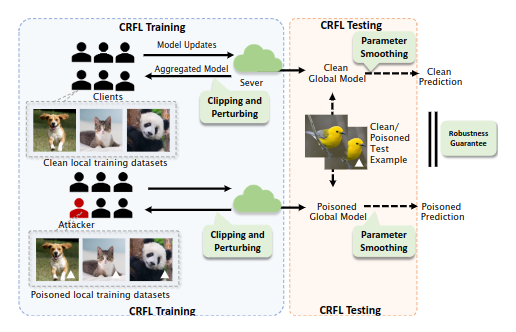
\includegraphics[width=0.8\linewidth,height=0.6\linewidth]{picture/CRFL.png}}
    \caption{Overview of certifiably robust federated learning (CRFL). CRFL controls the model smoothness through pruning and smoothing of model parameters and generates sample robustness
    certification against amplitude-limited backdoor attacks. Smoothness and perturbation methods are also used as 
    additional components to constrain the L2 norm of individual updates to enhance defense performance}
    \label{fig11}
\end{figure}


Considering that all of the above defense works lack robustness certification,
Xie et al. \cite{b86} proposed the first general defense framework CRFL for training certifiably robust FL models against backdoor attacks.
As shown in Fig.\ref{fig11},CRFL controls the model smoothness through pruning and smoothing of model parameters and generates sample robustness
certification against amplitude-limited backdoor attacks. Smoothness and perturbation methods are also used as
additional components to constrain the L2 norm of individual updates to enhance defense performance \cite{b87}.

In addition, the FL-WBC \cite{b88} method aims to identify the fragile parameter space in FL and perturb it
during client training. FL-WBC also provides robustness guarantees against backdoor attacks and convergence guarantees for FedAvg.
These developments demonstrate promising steps towards improving FL's robustness against backdoor attacks. In FLARE \cite{b89}, a trust
evaluation method is proposed that calculates a trust score for each model update based on the difference between all model updates and
their penultimate layer representation values. FLARE assumes that most clients are trustworthy and assigns low scores
to updates that are far from benign update clusters. The model updates are then aggregated with their trust scores as
weights and the global model is updated accordingly.

In \cite{b98}, the concept of anti-backdoor learning is introduced, which involves training a clean model given infected data,
dividing the overall learning task into a dual task of learning the clean part of the data and the backdoor part.
The article leverages two inherent weaknesses of backdoor attacks: models learn backdoor data faster than clean data,
and the stronger the attack, the faster the model converges on the backdoor data. Additionally, backdoor tasks are mutually
associated with specific classes. Based on these two weaknesses, a generic learning scheme is proposed to automatically prevent
backdoor attacks during training. A two-stage gradient ascent mechanism is introduced to isolate and separate backdoor samples
from the target class during the early training stage and break the association between backdoor samples and the target class during the later training stage.
\subsubsection{Model Reconstruction}
The model reconstruction-based approach aims to eliminate hidden backdoors in infected models by directly modifying suspicious models.
Therefore, even if triggers are included in the attack samples, the reconstructed model will still correctly predict them because
the hidden backdoors have been removed.

As mentioned earlier, the forgetting mechanism of federated backdoor attacks means that as training and model aggregation progress,
the backdoor will be forgotten in successive iterations. As a defense, this forgetting mechanism can also be utilized to create many defensive methods.

Zeng et al. \cite{b90}defined multiple training as a min-max problem and used implicit hyper-gradients to
explain the interdependence between internal and external optimization.
In \cite{b91}, Zhao et al. showed that hidden backdoors infecting DNNs can be repaired using pattern connectivity techniques with a certain number of benign samples.

Li et al. \cite{b92} perturbed backdoor-related neurons based on the distillation process, reconstructed (infected) DNNs using knowledge
distillation techniques , and thus removed hidden backdoors.
Huang et al. \cite{b109} proposed a distillation technique that utilizes Cognitive Distills to extract Cognitive patterns.
This is because the patterns of backdoor examples are generally small and sparse, making it possible to detect poisoned examples.


In addition to directly eliminating hidden backdoors, defense based on trigger synthesis first
synthesizes backdoor triggers, and then in the second phase, eliminates hidden backdoors by suppressing the influence of triggers.
These defenses have some similarities in the second phase with reconstruction-based defenses. For example,
pruning and retraining are commonly used techniques to remove hidden backdoors in both defenses. However,
compared to reconstruction-based defenses, the trigger-based defenses' trigger information makes the removal process more effective and efficient.

A GAN-based method was proposed in \cite{b93} to synthesize trigger distributions.
In \cite{b94}, they showed that the detection process used in \cite{b95} to determine synthesized
triggers has several failure modes and proposed a new defense method based on this observation.
Additionally, Cheng et al. \cite{b96} revealed that the $\infty$ norm of activation values can be used to
distinguish backdoor-related neurons based on synthesized triggers. Therefore, they proposed performing an
∞-based neuron pruning to remove neurons with high activation values in response to triggers.
Similarly, Aiken et al.\cite{b97} also proposed removing hidden backdoors
by pruning DNNs based on synthesized triggers from another perspective.

In general, we do not consider filtering techniques to be a viable solution for mitigating backdoor attacks.
Because filtering technologies are generally designed for specific types of attacks, they can be easily spoofed by attackers.
Instead, we believe that the focus of research on backdoor defense should be on model reconstruction and robust training.

\section{Byzantine Attack}
The Byzantine attack is a malicious attack that typically occurs in distributed systems with malicious participants. 
In the field of computer science and cryptography, the Byzantine Generals Problem describes the scenario of distributed systems with malicious participants. 
The essence of the Byzantine Generals Problem lies in how to achieve consensus among all nodes in the system when facing potential malicious participants.

Byzantine attacks pose a significant threat to the security and reliability of distributed systems. 
This chapter focuses on categorizing Byzantine attacks into three types and provides an overview of the challenges faced and future directions for development.

The first type of Byzantine attacks is the Sybil attack. It was first proposed by John Douceur in 2002 \cite{b110}. 
As shown in Fig.\ref{fig12},it is a type of network security attack where the attacker creates multiple fake identities or nodes to undermine the network's trust mechanism and disrupt its normal operation.

The principle behind this attack is that the attacker creates a large number of fake identities, nodes, or accounts that appear independent and genuine to the network but are actually controlled by the attacker. 
The attacker can use various means to create these fake entities, including using forged IP addresses, anonymous proxy servers, virtual machines, and more. 

\begin{figure}[htbp]
    \centerline{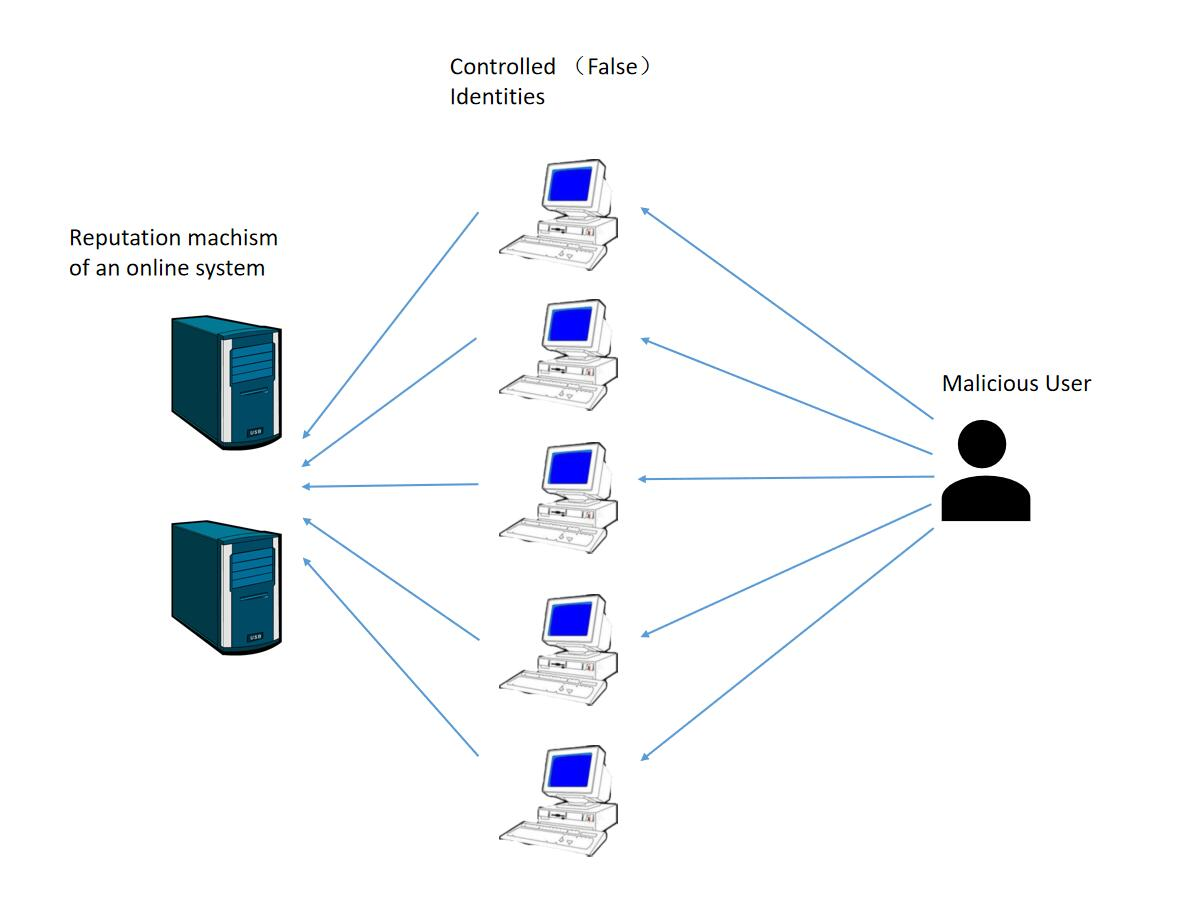
\includegraphics[width=0.8\linewidth,height=0.6\linewidth]{picture/sybil.jpg}}
    \caption{The schematic of the Sybil attack. Malicious users create a large number of fake nodes and control them to disrupt the normal operation of the network}
    \label{fig12}
\end{figure}

This attack mainly targets systems that rely on trust and identity verification mechanisms, 
such as peer-to-peer networks, social networks, and blockchains. Attackers can use a large number of fake identities to control the resources of the system, deceive other users,
and disrupt consensus mechanisms. For example, in a peer-to-peer network, attackers can create numerous fake nodes to control the distribution process of files,
leading to uneven resource distribution or network performance degradation.

The Sybil attack has posed significant threats to various network security systems since it was 
proposed. Bhagoji \cite{b111} explored some attack strategies against deep neural networks by enhancing 
malicious agent updates and employing alternating minimization strategies for stealth and adversarial 
targets. They demonstrated the possibility of effective and covert model poisoning attacks. 
Jun  \cite{b112} and others were the first to explore the Freerider attack in federated learning and proposed 
an incremental weight attack method that can evade most defense monitoring methods at that time. 
They also introduced a new high-dimensional anomaly detection method called STD-DAGMM, which is 
particularly useful for detecting freeriders. This method has potential applications for detecting 
other models' weight anomalies as well, which will be discussed in the next chapter.

In recent years, Sybil attacks have undergone significant development. 
Attackers employ more advanced techniques to create false identities, making Sybil nodes 
more realistic and difficult to distinguish.For instance, they might use virtualization technology
to create multiple independent virtual machines, each with its own IP address and network identifier.
Attackers can also utilize social engineering tactics and information acquisition methods to disguise 
themselves as genuine users or obtain additional fake identities through the authorization of l
egitimate users. Furthermore, attackers might construct more complex and realistic Sybil networks 
by leveraging shared information in social networks. 

Haonan Yang \cite{b113} focused on the problem of vehicular ad hoc networks and criticized previous 
studies for only considering the security threats and impacts of Sybil attacks in VANETs without 
analyzing the potential threats and impacts in VFCs (Vehicular Fog Computing). 
Therefore, the author summarized four types of Sybil attacks that could affect VFCs in areas such 
as routing, vehicle decision-making, voting, and reputation systems.

With the widespread use of mobile devices and the wireless networks, Sybil attacks have also 
started to increase in these environments. Attackers can threaten the security of location services, 
social networks, and mobile applications by utilizing false identities and location information on
 mobile devices. In the future, Sybil attacks can be more extensively applied to blockchain 
 technology, which enable attackers to manipulate consensus algorithms, launch double-spending 
 attacks, or undermine the fairness of blockchain networks by controlling a large number of 
 counterfeit identities.

 The second type of Byzantine attacks is based on the transmission process. Byzantine attacks can 
 occur during the communication process between participants. Attackers can tamper with, delete, or 
 insert malicious messages to disrupt the transmission of model updates.

Linyuan Zhang \cite{b114} proposed a centralized related probability small-scale attack (CDPS), 
which utilizes additional information. For instance, fusion rules in fault diagnosis \cite{b115} can be 
considered as existing knowledge usable for optimizing attack tactics. One form of CDPS attack 
involves collaborative efforts among malicious users who engage in communication. Moreover, sharing 
of information can assist malicious users in devising efficient attack strategies. Generally, 
colluding malicious users \cite{b116},\cite{b117} first exchange measurement values to ensure more accurate decisions 
on the licensed channel state and then report the coordinated forged results to enhance attack power. 
Moreover, Omid Fatemieh introduced another attack model called the full-knowledge attack \cite{b118}.

Cooperative spectrum sensing (CSS) is considered a promising method for identifying available 
spectrum. However, it not only requires a significant amount of communication resources but also 
introduces vulnerabilities to Byzantine attacks. Jun Wu \cite{b119} mentioned that attackers keep reporting 
false information to the fusion center consistently. In fact, attackers may attack discontinuously
 while appearing normal during rest periods. The author proposed a low-complexity sequential 0/1 
 (S0/1) method for CSS in the presence of strategic Byzantine attacks. It does not require strong 
 assumptions or any prior knowledge, and this method will be discussed in the next chapter.

 With the development of IoT devices, attackers may exploit communication vulnerabilities and 
 weaknesses between IoT devices to launch future attacks. Attackers may also utilize high-speed, 
 low-latency 5G/6G networks to carry out larger-scale distributed denial-of-service (DDoS) attacks,
  bypass security measures using network slicing and virtualization technologies, or exploit 
  vulnerabilities in mobile communication protocols to attack devices and systems.

  The third type of Byzantine attacks is known as model aggregation attack. In this type of attack, 
  Byzantine attackers manipulate the model parameters of the participants in order to influence the 
  aggregation results. 
  
\begin{figure}[htbp]
    \centerline{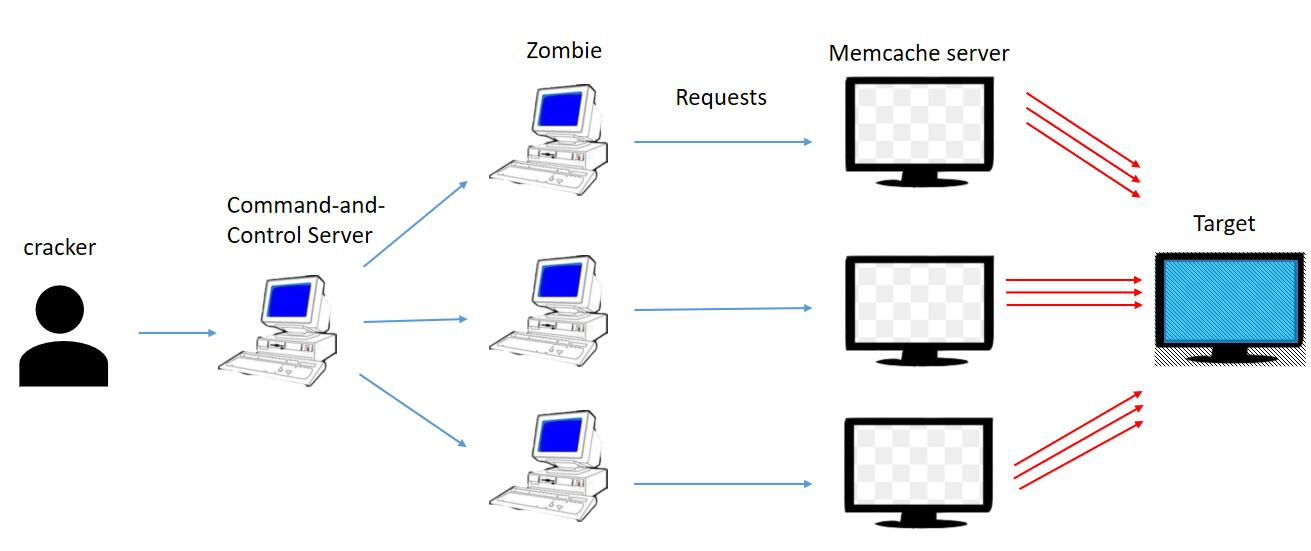
\includegraphics[width=0.8\linewidth,height=0.6\linewidth]{picture/ddos.jpg}}
    \caption{The schematic of a DDOS attack. Through the central control system, the attacker uses specific software or malicious code to remotely control multiple zombies, making them send a large number of requests to the target system at the same time to exhaust the processing power, network bandwidth or resources of the target system, thus causing the target system to fail to work normally}
    \label{fig13}
\end{figure}

As discussed by El Mhamdi \cite{b120}, these attacks by Byzantine workers may not 
prevent the model from converging but can instead lead to convergence on suboptimal solutions. 

Cong Xie \cite{b121} proposed a form of attack called Gamber. In this attack, an attacker can modify 
some of the data communicated between participants. The attacker randomly selects data and makes 
malicious changes to them. 

A different type of attack is called omniscient.
The attacker needs to have knowledge of the gradients sent by all the staff members.
The attacker then replaces some gradient vectors by taking the sum of all gradients, scaled by 
large negative values.

The objective is to mislead the Stochastic Gradient Descent (SGD) algorithm into moving in the opposite direction with larger step sizes.

Weaker attacks, such as Gaussian attacks, are also possible.In these attacks, some gradient vectors are replaced with random vectors sampled from a Gaussian distribution that has a large variance.
Such attackers do not require any information from the staff members.

\begin{figure}[htbp]
    \centerline{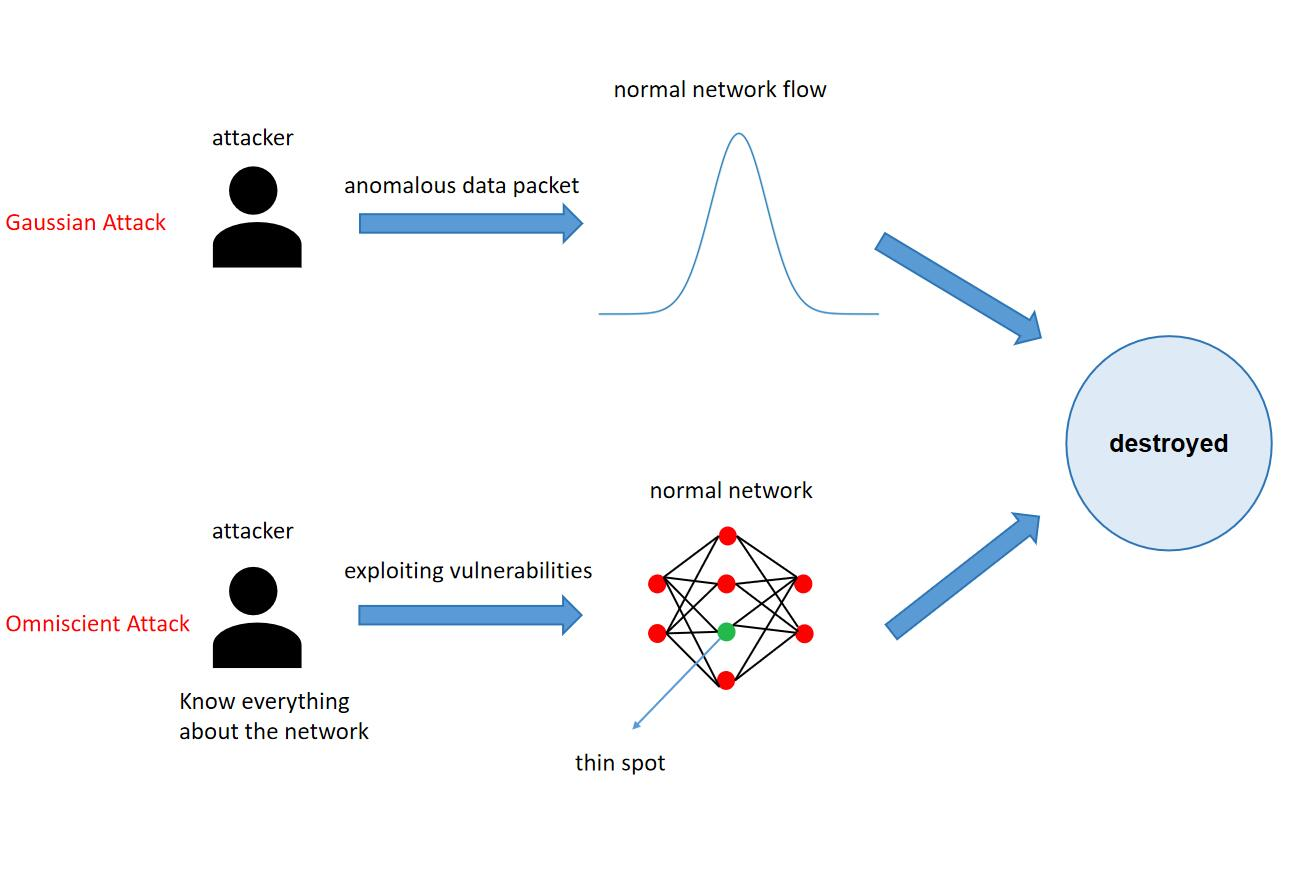
\includegraphics[width=0.8\linewidth,height=0.6\linewidth]{picture/gause.jpg}}
    \caption{The schematic of Gaussian attack and Omniscient attack.In a Gauss attack, an attacker enters incorrect packets into the network, affecting the normal running of network flows.An omniscient attack is a hypothetical scenario where an adversary has complete and perfect knowledge or awareness of the system they are targeting. In this type of attack, the adversary has access to all the information and capabilities necessary to exploit vulnerabilities in the system. With this all-encompassing knowledge, the attacker can strategically plan and execute attacks to maximally exploit the system’s weaknesses.
    }
    \label{fig14}
\end{figure}

In many applications, multiple sources can provide descriptions of the same object or event, which 
can inevitably lead to conflicts in data or information. Resolving conflicts in data is an important
challenge in achieving convergence in federated learning. Byzantine attackers have the ability to 
exploit these issues in order to manipulate the convergence of the model. 
Qi Li \cite{b122}, Harry Hsu \cite{b123}, and Yanna Jiang \cite{b124} have all explored questions related to data differences and conflicts.
 
In future attacks, attackers may attempt to achieve their objectives by making modifications to the 
trained model. This can involve incorporating backdoors into the model, which would produce 
incorrect outputs under specific conditions, or tampering with the model parameters to disrupt its robustness. 

In order to evade detection, future attack strategies could involve the development of more advanced 
and covert techniques to camouflage malicious modifications. Additionally, malicious insiders who 
have access to the model parameters may exploit this privilege to launch attacks. They could
manipulate the parameters to compromise the model's performance or even insert sensitive
information within the model itself.

In the coming years, attackers may explore more complicated techniques and algorithms to 
bypass security monitoring and detection mechanisms. The aim would be to implement internal
personnel attacks more efficiently. These advancements would allow attackers to bypass 
existing safeguards and carry out their malicious activities with greater precision and 
effectiveness.


\section{Defenses against Byzantine Attack}

With the advancement of Byzantine attacks, the corresponding defense methods are constantly evolving and being updated.
Based on the different types of Byzantine attacks discussed in the previous chapter, we categorize the Byzantine defense methods into three classes:

For Sybil attacks, the defense methods include trust-based evaluation methods and machine learning models for detecting fake nodes.

Stephanie Gil \cite{b125} proposed a novel algorithm that analyzes received wireless signals to 
detect the presence of deceptive clients created by adversaries. It does not require specialized
hardware or private key exchanges; commercial Wi-Fi cards and software are enough. It utilizes 
the physical characteristics of wireless signals to "perceive" deceivers. The author conducted 
experiments using the AscTec quadcopter server team and iRobot Create ground clients, which show 
that a deception detection rate exceeding 96%.


Blanchard et al. \cite{b126} introduced Krum, which detects and removes outliers in gradient aggregation, allowing convergence
even in the presence of multiple Byzantine attackers, and with low complexity.

Luis Muñoz-González \cite{b127} proposed a new algorithm for robust federated learning called 
Adaptive Federated Averaging, aiming to detect faults, attacks, and malicious updates provided 
by participants in a collaborative model. The author also proposed a Hidden Markov model to simulate
and learn the quality of model updates provided by each participant during training.

\begin{figure}[htbp]
    \centerline{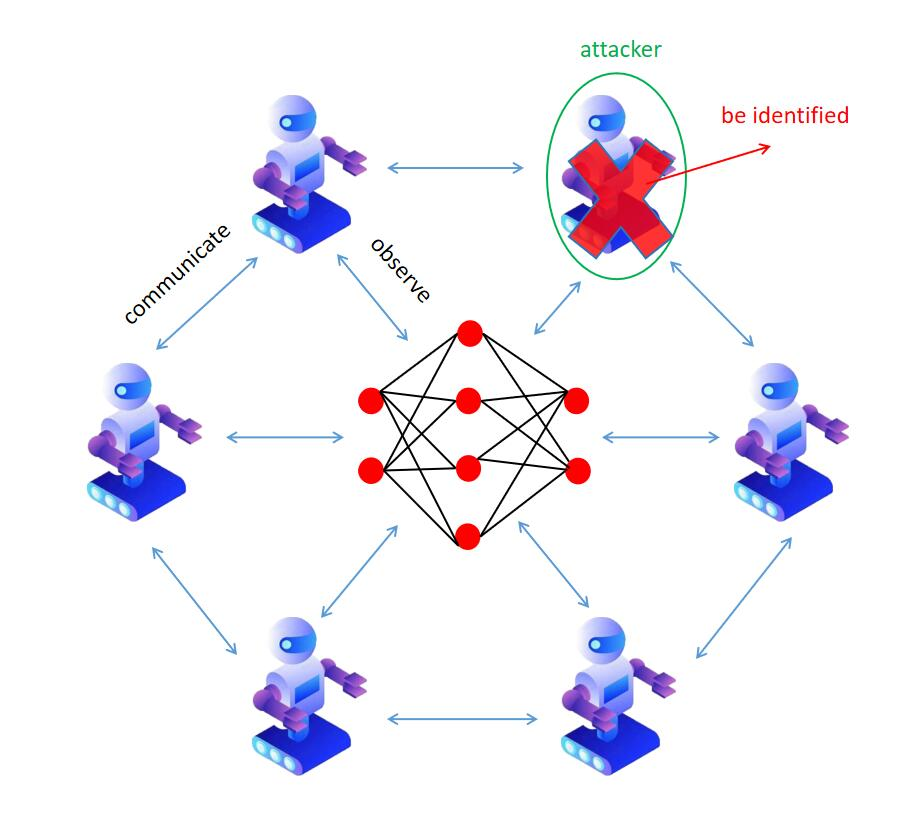
\includegraphics[width=0.8\linewidth,height=0.6\linewidth]{picture/robot.jpg}}
    \caption{Robots can communicate with neighbors to get information, combined with their own information, in a certain round can eliminate the interference of malicious robots, reach a consensus.}
    \label{fig15}
\end{figure}

Defense methods against Sybil attacks in robot networks have also seen rapid development. 
In Frederik Mallmann-Trenn's work \cite{b128}, a combination of wireless signal analysis and 
observations from sociological learning was used to demonstrate rapid convergence of correct trust 
values for all robots in the team when facing attacks. All robots develop their own opinions 
about network trust by observing messages sent through the network as shown in Fig.\ref{fig15}. They 
then compare their opinions with those of their neighbors to reach a consensus on whether the 
robots can be trusted. By utilizing their neighbors' opinions, each robot effectively increases 
the number of observations available to them about the network, thereby eliminating messages with 
a high probability of coming from malicious robots through cross-validation. Experiments showed 
that in a limited number of communication rounds, all robots agreed on the global consensus of 
trustworthiness in their neighborhood.

Sybil attacks pose a significant challenge as attackers can create a large number of false 
identities, making it difficult to detect and differentiate them. Therefore, developing 
secure systems requires consideration of multiple defense methods and selecting appropriate
solutions based on specific application contexts. 

The future outlook for such defense techniques primarily focuses on the following areas:
enhancing identity verification mechanisms to distinguish genuine users from Sybil nodes 
and establishing stronger trust mechanisms to identify and filter out Sybil nodes displaying
malicious behavior. In recent years, the emergence of blockchain technology has provided a 
decentralized, tamper-resistant, and secure shared ledger, offering a potential defense against 
Sybil attacks. By combining identity verification, trust mechanisms, and blockchain technology, 
the ability to detect and prevent Sybil nodes can be improved.


Defense methods against attacks during the transmission process include designing secure communication protocols and encryption mechanisms.

Previous malicious detection and suppression algorithms focused only on simple "always attack" 
scenarios, where attackers continuously report false information to the central entity. 
In reality, attackers may intermittently attack while behaving normally at other times. 
Under the assumption of simple attack strategies, Ruiliang Chen \cite{b129} proposed sequential hypothesis
testing to defend against Byzantine attacks, but it requires significant computation and prior 
knowledge. 

Therefore, Jun Wu \cite{b119} introduced S0/1 using support vector regression (SVR) to offset 
strategic Byzantine attack defense. Even in a blind scenario, this approach greatly reduces the 
sample size while providing higher correct sensing ratios.


Luis Muñoz-González \cite{b127} alsoproposed a robust aggregation rule that detects and discards malicious or poor local model updates during each training iteration. It includes mechanisms for blocking unwanted participants, thereby enhancing computational and communication efficiency.
In traditional federated learning, the performance of models may decline due to variations in data distributions across devices. 

To address this issue, Hesham Mostafa (7) proposed a technique called "representation matching." 
This technique improves model performance by matching features between the global model and 
local models. For clients with homogeneous data distributions, this approach consistently 
improves accuracy. For heterogeneous clients, in addition to improving accuracy, this approach 
enhances training robustness and avoids catastrophic training failures without the need for manual 
hyperparameter tuning for each task.

\begin{figure}[htbp]
    \centerline{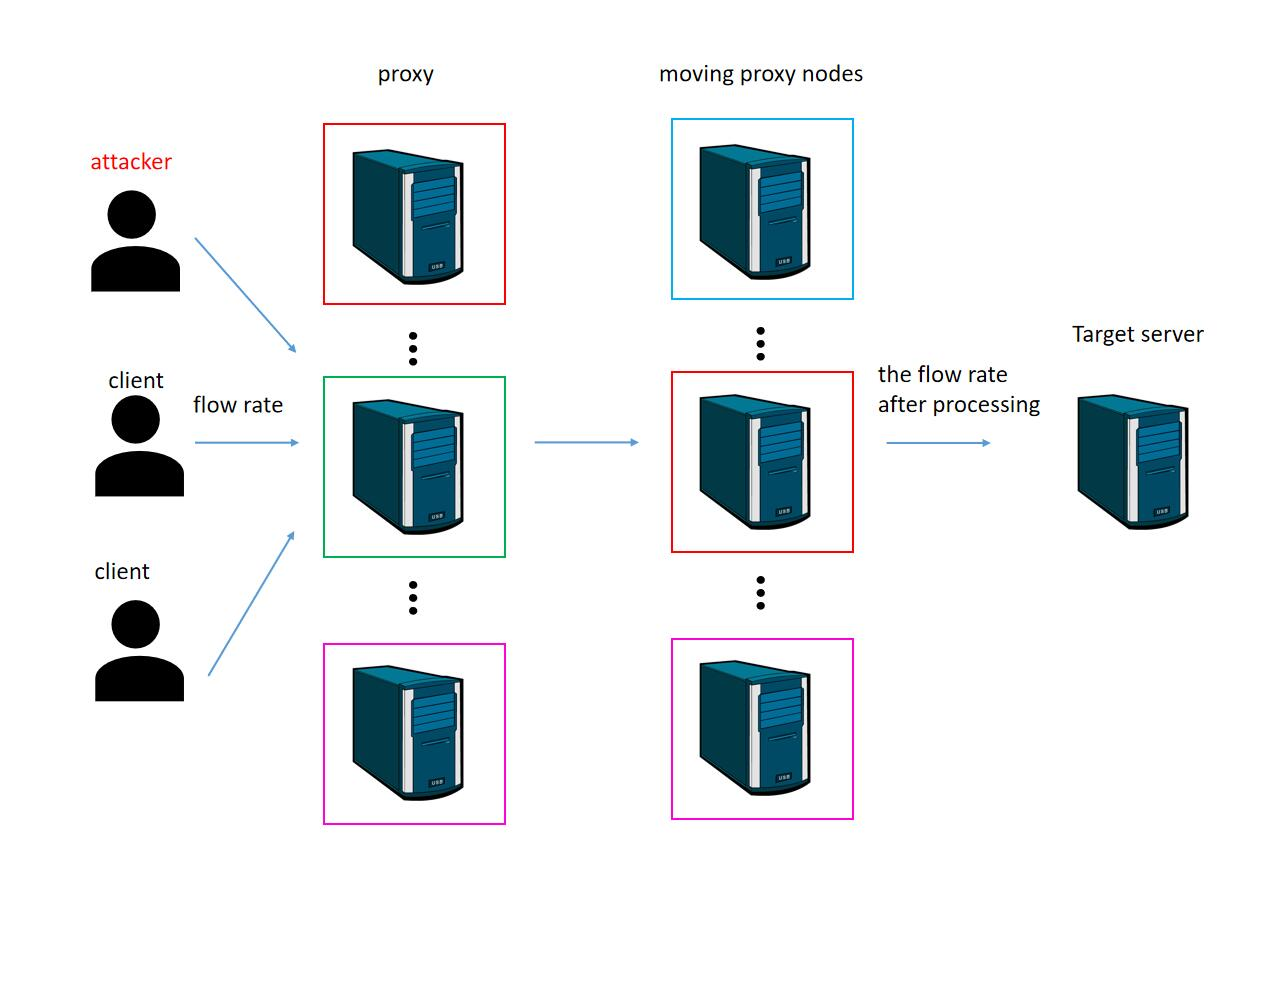
\includegraphics[width=0.8\linewidth,height=0.6\linewidth]{picture/de-ddos.jpg}}
    \caption{DDOS defense method of secret moving proxy nodes.The proxy node is constantly moving its position, confusing the attacker so that it cannot find the real target server}
    \label{fig16}
\end{figure}

Huangxin Wang \cite{b131} proposed a mobile target defense mechanism that specifically addresses DDoS
attacks targeting authenticated clients of Internet services.
This mechanism utilizes a set of dynamic and hidden proxies to relay
traffic between authenticated clients and servers. As shown in Fig.\ref{fig16}, by continuously
replacing the attacked proxies with backup proxies and reallocating attacked clients to new proxies,
innocent clients are separated from malicious insiders through a series of shuffling.
In recent years, significant efforts have been made in defending against
low-rate DDoS attacks. Attackers easily launch complex low-rate
DDoS attacks by exploiting prominent features of cloud computing.
Therefore, research on various DDoS attacks and their corresponding defense
methods is crucial in protecting cloud infrastructure from devastating impacts
of DDoS attacks. Neha Agrawal \cite{b132} conducted a comprehensive classification
of all possible variants of cloud DDoS attack solutions and provided detailed insights
into characterization, prevention, detection, and mitigation mechanisms.

In the future, these defense methods can be further developed by constructing more secure and
robust encryption protocols and algorithms. Additionally, more effective Identity verification 
technologies can be developed to ensure the trustworthiness of communication parties. Continual 
improvement and enhancement of transport layer protocols, such as SSL/TLS, can provide stronger 
security and defense capabilities, including the ability to resist man-in-the-middle attacks, 
data tampering, and replay attacks. The development of real-time threat detection systems capable 
of detecting and responding to attacks during the transmission process can also be explored.With 
the advancement of quantum computing, traditional encryption algorithms may be threatened. 

Therefore, researching and developing quantum-safe communication protocols and algorithms is also 
important to ensure security during the transmission process and protect data confidentiality in a 
quantum computing environment.

Defense methods against model aggregation attacks include designing robust aggregation 
algorithms and using differential privacy techniques to protect model parameters.


Qi Li \cite{b122} modeled the problem using an optimization framework where ground 
truth and source reliability are defined as two sets of unknown variables. The objective 
is to minimize the overall weighted differences between the ground truth and multiple-source 
observations, with each source weighted by its reliability. This framework can incorporate 
different loss functions to identify features of various data types and has developed efficient 
computing methods that effectively identify the true information among conflicting data sources.


El Mahdi El Mhamdi \cite{b120} argues that mere convergence of the Byzantine resilient 
rules is not enough. It is possible that Byzantine workers' attacks can lead to convergence 
to the worst suboptimal solution. To address this, he proposes a generic enhancement method 
called Bulyan. This method significantly reduces the leeway for Byzantine workers, constraining 
them within narrow boundaries. For common batch sizes, Bulyan achieves performance comparable to 
average speed.

Cong Xie \cite{b121} introduces three robust aggregation rules for stochastic gradient 
descent (SGD) with low computational costs. These rules are the first to be theoretically 
and empirically studied under the non-convex setting, based on median aggregation.

Harry Hsu \cite{b123} presents a method for synthesizing datasets with continuous identical 
ranges and provides performance metrics for the federated averaging algorithm. Experimental 
results demonstrate that performance deteriorates with distribution differences. The proposed 
method suppresses oscillations through the accumulation of gradient history, and it has been 
shown that using momentum on top of SGD for non-iid problems has achieved significant success 
in accelerating network training.


Amit Portnoy \cite{b133} proposes a novel method called Byzantine Robust Client Weighting (BRCW) to 
minimize the impact of malicious clients in federated learning. BRCW assigns different weights to 
each client based on their credibility and contribution to the overall model accuracy. 
During training, the weights are dynamically updated according to each client's performance 
and behavior. Unlike previous work, this study considers the sample size provided by clients 
as untrustworthy, as it may come from malicious clients. BRCW exhibits robustness against various 
forms of attacks, including communication disruptions and data poisoning.

Krishna Pillutla \cite{b134} designs a novel robust aggregation oracle based on classical 
geometric medians and demonstrates its robustness in federated learning with limited heterogeneity, 
even when up to half of the devices are faulty. The proposed RFA algorithm outperforms the standard 
FedAvg (14) in high damage scenarios and nearly matches FedAvg's performance in low damage scenarios, 
but with 1-3 times higher communication costs.

\begin{figure}[htbp]
    \centerline{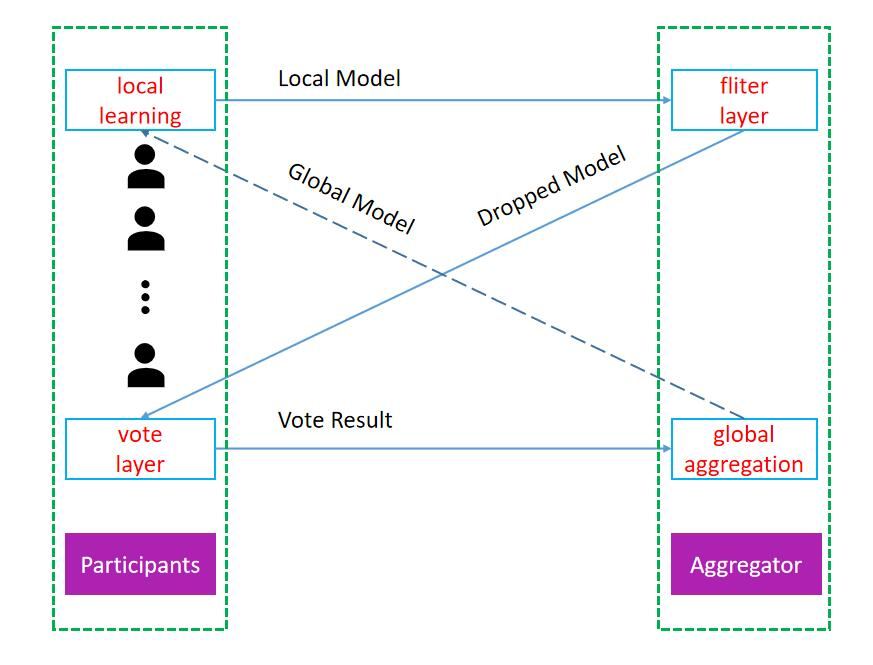
\includegraphics[width=0.8\linewidth,height=0.6\linewidth]{picture/vote.jpg}}
    \caption{The structure of two-layer aggregation method.Participants share the global model, and models discarded by the filter layer are not directly abandoned, but are voted by participants to participate in the final aggregation process.}
    \label{fig17}
\end{figure}

Yanna Jiang \cite{b124} introduces the combination of handling imbalanced data and Byzantine attacks 
in the context of federated learning for the first time. The concept of an intelligence pool is 
proposed to separate the task of judging the shared local model values from the aggregator, 
avoiding the limitations of a single criterion through two-layer verification shown in Fig.\ref{fig17}.

Future prospects for such defense methods will focus on more stricter authentication 
and authorization mechanisms, as well as parameter integrity protection. Mechanisms such 
as Hash algorithms or digital signatures can be adopted to safeguard the integrity of parameters, 
preventing tampering during transmission and storage. 

Detection of malicious parameter modifications and corresponding response measures are also required. 
By comprehensively applying these methods, the defense capability against malicious parameter 
modification attacks can be enhanced, ensuring the security and integrity of systems and applications.




\section{Adversarial Attack}  

Both adversarial attacks and backdoor attacks are techniques used to modify benign testing samples
in order to make models misbehave during the inference process. While adversarial perturbations are sample-agnostic in universal adversarial attacks,
these attacks can appear similar to backdoor attacks. Consequently, researchers who are unfamiliar with backdoor attacks may question their significance,
as these attacks require additional controls on the training process to some extent.
However, despite certain similarities, these attacks have essential differences.

Firstly, adversarial attackers need to control the inference process to a certain degree
but not the training process of models. They must query the model results or even gradients multiple
times to generate adversarial perturbations by optimization, given a fixed targeted model.
On the other hand, backdoor attackers require modifying certain training stages,
such as data collection and model training, without any additional requirements in the inference process.
Secondly, from the perspective of attacked samples, backdoor attackers use known,
non-optimized perturbations, whereas adversarial attackers require obtaining
them through the optimization process based on the model output.
This optimization in adversarial attacks requires multiple queries,
making them unable to be real-time in many cases.
Finally, the mechanisms of these attacks are fundamentally different.
Adversarial vulnerability results from the differences in behaviors of models and humans,
while backdoor attackers exploit the excessive learning ability of deep neural networks (DNNs)
to establish a latent connection between trigger patterns and target labels.

In federated learning, because the data is not shared among participants,
attackers can use this to generate adversarial samples locally,
then inject them into the data sets of participants, and train
the model with the data of other participants during the training process.

So, how should attacks targeting federated learning be designed?
In centralized learning, FGSM\cite{b99} was initially used to generate adversarial examples.
Let $\theta$ be the parameters of a model, $x$ the input to the model,
$eta$ the perturbation to original input and $||\eta||_\infty \le \epsilon$,
$y$ the targets associated with $x$ (for machine learning tasks that have targets)
and $J(\theta, x, y)$ be the cost used to train the neural network.
We can linearize the cost function around the current value of $\theta$,
obtaining an optimal max-norm constrained pertubation of:
\begin{equation}
    \eta = \epsilon sign(\nabla_x J(\theta,x,y))
\end{equation}

In federated learning, attackers can use FGSM locally to generate
adversarial samples and then inject them into the datasets of some participants
to affect the performance of the entire model.

PGD\cite{b100} is a more powerful adversarial sample generation method,
which generates adversarial samples by iteratively perturbing the input.
Specifically, PGD first randomly generates an initial disturbance $\delta_0$,
and then iteratively updates the disturbance $\delta_t$, to meet the constraint,
that is, $|\delta_t|_{\infty} \leq \epsilon_{\text{max}}$,
where $\epsilon_{\text{max}}$is the maximum value of the disturbance.
After each update, PGD also projects the disturbance
$\delta_t$ back into the constraint space to ensure that it meets the
constraint conditions.
Specifically, the update formula for PGD is as follows:
\begin{equation}
    x^{t+1} = \text{Clip}(x + \text{sign}(\nabla_x L(\theta,x',y)) \cdot \epsilon{\text{max}}, x - \epsilon_{\text{max}}, x + \epsilon_{\text{max}}),
\end{equation}
Where $\text{Clip}$ means to cut $x$ into the interval, and $\epsilon_ {\text{max}} $is the maximum value of the disturbance.
Unlike FGSM, PGD requires multiple iterations to generate adversarial examples,
so attackers need to use the local dataset and model parameters of each participant
to iteratively update the perturbation.

In federated learning, using PGD (Projected Gradient Descent) or FGSM
(Fast Gradient Sign Method) to generate adversarial examples and perform
adversarial attacks is a common method. However, compared to centralized
learning, there are some considerations and techniques that need to be
taken into account.

\subsubsection{Data privacy and distribution heterogeneity}: In federated learning, data is
typically distributed across various edge devices, making it slightly more
difficult to generate adversarial examples and perform attacks. Therefore,
attackers need more complex strategies to adapt to the heterogeneity of the
data distribution. In this case, the generation of adversarial examples should
consider the data distribution and usage on each device. In federated learning,
the amount and quality of data from each participant may vary, leading to
imbalanced training data. This may affect the effectiveness of adversarial attacks,
as attackers may not be able to generate sufficiently accurate adversarial
examples to attack all participants' models.

\subsubsection{Network latency and bandwidth limitations}: In federated learning,
devices communicate through a network, which may result in network
latency or bandwidth limitations. Therefore, when generating adversarial
examples and performing attacks, these factors need to be taken into
consideration. For example, it may be necessary to optimize the size
and generation speed of adversarial examples to adapt to network limitations.
And in federated learning, the training steps of each participant are asynchronous,
which may lead to synchronization issues. For example, attackers may not be able
to perform attacks on all participants' models because they may be at
different training steps or states.

\subsubsection{Update of attack strategies}: Due to the dynamic nature of federated
learning, attackers need to constantly update their attack strategies
to adapt to changes in the learning model and data distribution. This
may require designing more complex attack strategies and using more
efficient optimization algorithms.

\subsubsection{Attack detection and defense}: In federated learning, adversarial
attacks may be easier to detect due to the distribution and usage
of data. Therefore, it is necessary to design adversarial examples
that are more difficult to detect or use more complex attack strategies
to avoid detection.

Overall, using PGD or FGSM to generate adversarial examples and perform
adversarial attacks in federated learning requires considering the
characteristics and limitations of federated learning, including
the heterogeneity of data distribution, network latency and bandwidth
limitations, update of attack strategies, and attack detection and defense.
This may require designing more complex and efficient attack strategies
and adversarial example generation methods.


\section{Defenses against Adversarial Attack}

Overall, progress has been made in defending against adversarial samples.
As adversarial samples share similarities with the previously discussed backdoor
samples, defense methods involving sample filtering can be employed.
However, in this section, we will refrain from discussing filtering methods
and instead focus on the defense method of adversarial training.

Adversarial training is a defense method against adversarial attacks.
Its basic idea is to incorporate adversarial examples into the training process,
enabling the model to better withstand unknown adversarial attacks.
Specifically, adversarial training combines the original training dataset
with adversarial samples generated to target the model, and retrains the
model accordingly. This way, the model encounters adversarial examples
continuously during the learning process, thereby enhancing its robustness
and generalization capability.

FAT (Federated Adversarial Training) is a method proposed in \cite{b31} that
combines federated learning and adversarial training to reduce evasion
threats during inference while preserving data privacy during training.
In the FAT protocol, each device trains a local model and generates adversarial
samples, which are mixed with the original data for training.
The models are then uploaded to the server for aggregation.
This helps to improve the robustness of the model against adversarial attacks.
The authors note that the protocol does not work out of the box and requires careful
tuning of the optimization parameters to achieve good results. Additionally, the authors
acknowledge that the experiments were conducted on idealized federated settings and that
further research is needed to evaluate the effectiveness of FAT in more realistic scenarios.

So, there are also several challenges with implementing adversarial training in federated learning,
such as heterogeneous clients caused by distribution, certified guarantees, privacy leakage, slow convergence rate.


\subsection{heterogeneous clients caused by distribution}  
The major challenge in federated learning is the heterogeneity of clients.  
This means that the distribution of training data may vary among different clients, 
and the computational resources available to each client may also differ.
The paper\cite{b101} proposes a novel method called FedRobust to address the problem of
distribution shifts in federated learning. FedRobust is a gradient descent ascent
(GDA) algorithm that solves the minimax robust optimization problem and can be
efficiently implemented in a federated setting. This paper show that FedRobust,
which alternates between the perturbation and parameter model variables,
will converge to a stationary point in the minimax objective that satisfies
the Polyak-Łojasiewicz (PL) \cite{b102} condition. This optimization method can be used
to address the issue of distribution shifts in federated learning,
which can significantly impact the performance of the trained model.


\begin{figure}[htbp]
    \centerline{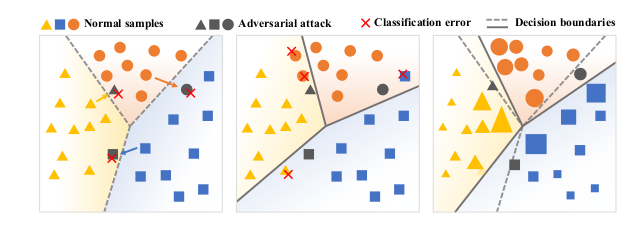
\includegraphics[width=1.0\linewidth,height=0.4\linewidth]{picture/db.png}}
    \caption{Decision boundary of DBFAT-trainedmodel}
    \label{fig19}
\end{figure}

Zhang et al.\cite{b34} found that the accuracy of the federated learning model with
adversarial training decreases on clean data, especially when the data of different
client are non-independent and identically distributed, so they propose an algorithm
based on decision boundary as shown in Fig.\ref{fig19}, which uses local reweighting and global regularization
to improve the accuracy and robustness in federated adversarial training.
Chen et al.\cite{b32} studies the skewed labels problem in federated learning and proposes
a CalFAT framework to calculate the logits of each class. By using this framework, the models between different clients eventually converge, 
enhancing the robustness and accuracy of the global model.

Hong et al.\cite{b105} have studied the problems caused by clients with different computing resources.
During federated learning, some clients can support adversarial training, but some clients with
lack of computing resources can not support it. This paper studies how to spread resistance robustness
from resource-rich users who can support confrontation training to those users with poor resources.
This paper shows that an effective robust propagation algorithm is proposed by using BN layer technology correctly.  

\subsection{Certified Guarantees}  
Certified guarantees are needed in adversarial training to ensure reliable protection and security against unknown attacks in adversarial environments.
Certified guarantees refer to rigorous proofs and assurances of model performance. 
They provide protection bounds against specific types of attacks, 
indicating that the model can maintain a certain level of performance regardless of how carefully the attacker designs the attack, such as high accuracy or robustness.

By using certified guarantees, adversarial training can provide a degree of predictability and security. 
This means that in practical deployment, there is higher confidence in the model's performance and trustworthiness, 
rather than relying solely on trial-and-error evaluation and protection. 
It offers a more reliable and definitive defense mechanism for models to handle unknown or complex attacks.  

Chen et al.\cite{b104} proposes incorporating randomized smoothing techniques into federated adversarial
training to enable data-private distributed learning with certifiable robustness to test-time adversarial
perturbations. The experiments conducted in the paper show that this approach can deliver models as
robust as those trained by centralized training, and can enable provably-robust classifiers to
2-bounded adversarial perturbations in a distributed setup.

From the perspective of variance-bias decomposition,Chen et al.\cite{b108} decomposed the 
loss function into a combination of bias and variance, generated adversarial samples on the server 
and returned them to each client for adversarial training. Then, they used any model aggregation 
algorithm to improve the global model's adversarial robustness.

\subsection{Privacy leakage} 
As mentioned earlier, privacy protection is crucial in federated learning.
In \cite{b106},it is proved that the model of confrontation training is more prone to
privacy disclosure than the model of normal training.
Zhou et al.\cite{b103} argues that conventional federated learning frameworks are vulnerable
to strong adversarial attacks, even if adversarial training using locally
generated adversarial examples is performed on each client. To address this
problem, the paper proposes a new framework called FedBVA (Federated Learning
with Bias-Variance Analysis) that provides a tiny amount of bias-variance
perturbed data from the central server to the clients through asymmetrical
communication. This approach dramatically improves the robustness of the
training model under various settings, without violating the clients' privacy.

\subsection{Slow convergence rate}
As described in \cite{b34}, conducting adversarial training in federated learning is a challenging task because the convergence speed of adversarial training is very slow.
In \cite{b107}, a method was proposed to solve this problem.
Assuming the local iteration number of federated learning is E, this article believes that a larger E will
increase the drift between models and affect the adversarial robustness, but will converge quickly. A smaller
E will increase the adversarial robustness but decrease the convergence efficiency. Therefore, this article
proposes a dynamic mechanism for adjusting E, and uses FedCurv instead of FedAvg as the global aggregation
algorithm, and proposes a new algorithm called FedDynAT to simultaneously improve the convergence
speed and adversarial robustness.


\section{Advanced Research and Problems}

Recently, some works have studied the latent connection between adversarial attacks and backdoor attacks.
For example, Weng et al. \cite{b66}empirically demonstrated that defending
against adversarial attacks via adversarial training may increase the risks of backdoor attacks.
We can introduce sample filtering to prevent backdoor samples from entering the training dataset. 
Then, we can enhance adversarial robustness by introducing adversarial training on the client side. 
When sending gradient information to the server, we can perform malicious gradient filtering to construct a hybrid defense mechanism.
Model distillation can also serve as a hybrid defense mechanism. 
By training a more robust teacher model and using its output as labels to train a student model, 
model distillation can effectively mitigate the impact of backdoor attacks and adversarial sample attacks.
\subsection{Attack}  
Backdoor attackers need to effectively hide backdoors to make them difficult to detect.For example, by taking 
advantage of the distributed nature of federated learning, multiple clients can work together to inject backdoors into the global model.
Backdoor attackers should use different types of backdoors, such as hardcoding and model parameter optimization.  
This paper suggests that using generation techniques to create backdoor samples for dynamic attacks is a solution.
How to conduct persistent backdoor attacks is also a problem. 
One solution we give in this paper is to ensure that the injected backdoor can exist for a long time through edge samples, 
because the injected backdoor will be less affected by updates.

In Byzantine attacks,  how do Byzantine attackers leverage larger networks to launch attacks while evading detection is to be solved.  
Then how to make better use of the communication protocol vulnerability for device and system intrusion is also a key issue.

How to improve the transferability of adversarial samples.A possible solution is achieved by optimizing disturbances that affect common characteristics or patterns between different models.

\subsection{Defense}
In federated learning, client data is distributed among multiple participants. The protection of privacy is a important reason why federated learning is so popular. So it is an important challenge to ensure data privacy while implementing defenses.  
Detecting malicious participants quickly and accurately is also a key issue. Existing solutions rely mainly on consistency verification and anomaly detection, but there is still room for improvement in large-scale federated learning scenarios.  
Effective defense mechanisms, such as fault-tolerant algorithms and majority voting, are needed to counter Byzantine attacks. However, these mechanisms need to strike a balance with factors like privacy preservation and computational efficiency.
Adversarial training can enhance model robustness but may compromise generalization capability. Balancing the trade-off between adversarial robustness and generalization is a problem that requires exploration and resolution.
Designing models that can withstand zero-knowledge adversarial sample attacks remains an open question. It demands models to possess robustness without prior knowledge of adversarial samples during training.

Recently, some works have studied the latent connection between adversarial attacks and backdoor attacks.
For example, Weng et al. \cite{b66}empirically demonstrated that defending
against adversarial attacks via adversarial training may increase the risks of backdoor attacks.
We can introduce sample filtering to prevent backdoor samples from entering the training dataset. 
Then, we can enhance adversarial robustness by introducing adversarial training on the client side. 
When sending gradient information to the server, we can perform malicious gradient filtering to construct a hybrid defense mechanism.
Model distillation can also serve as a hybrid defense mechanism. 
By training a more robust teacher model and using its output as labels to train a student model, 
model distillation can effectively mitigate the impact of backdoor attacks and adversarial sample attacks.


\section{Conclusion}
In this survey, we systematically introduce state-of-the-art threats in federated learning systems,
which mainly include byzantine attacks, backdoor attacks and adversarial attacks. 
And we also detailed describe corresponding defensive policies.
We also introduce the advantages and disadvantages of these methods and how they work, and sort out the relationship between them.
Additionally, we discuss a number of open problems of current defense methods,
hoping them could help researchers identify and solve issues more quickly in the area of robust federated learning.



\newpage

\begin{thebibliography}{00}
    \bibitem{b1} Kirillov, Alexander, et al. "Segment anything." arXiv preprint arXiv:2304.02643 (2023).
    \bibitem{b2} M. Goddard, The EU General Data Protection Regulation (GDPR): European regulation that has a global impact, International Journal of Market Research 59 (2017) 703~705.
    \bibitem{b3} McMahan, Brendan, et al. "Communication-efficient learning of deep networks from decentralized data." Artificial intelligence and statistics. PMLR, 2017.
    \bibitem{b4} Q. Yang, Y. Liu, Y. Cheng, Y. Kang, T. Chen, H. Yu, Federated Learning, Synthesis Lectures on Artificial Intelligence and Machine Learning, 2019.
    \bibitem{b5} Doshi, Keval, and Yasin Yilmaz. Federated Learning-Based Driver Activity Recognition for Edge Devices.
    \bibitem{b6} Becking, Daniel, et al. Adaptive Differential Filters for Fast and Communication-Efficient Federated Learning. Apr. 2022.
    \bibitem{b7} Chen, Mingqing, et al. “Federated Learning of N-Gram Language Models.” Cornell University - arXiv,Cornell University - arXiv, Oct. 2019.  
    \bibitem{b8} Lin, BillYuchen, et al. FedNLP: A Research Platform for Federated Learning in Natural Language Processing. Apr. 2021.  
    \bibitem{b9} Liu, Rui, et al. "Federated graph neural networks: Overview, techniques and challenges." arXiv preprint arXiv:2202.07256 (2022).  
    \bibitem{b10} Wu, Chuhan, et al. "Fedgnn: Federated graph neural network for privacy-preserving recommendation." arXiv preprint arXiv:2102.04925 (2021).  
    \bibitem{b11} Guo, Shangwei, et al. "Robust and privacy-preserving collaborative learning: A comprehensive survey." arXiv preprint arXiv:2112.10183 (2021).
    \bibitem{b12} Enthoven, David, and Zaid Al-Ars. "An overview of federated deep learning privacy attacks and defensive strategies." Federated Learning Systems: Towards Next-Generation AI (2021): 173-196.
    \bibitem{b13} Rodríguez-Barroso, Nuria, et al. "Survey on federated learning threats: Concepts, taxonomy on attacks and defences, experimental study and challenges." Information Fusion 90 (2023): 148-173.
    \bibitem{b14} Tariq, Asadullah, et al. "Trustworthy Federated Learning: A Survey." arXiv preprint arXiv:2305.11537 (2023).
    \bibitem{b15} Zhang, Yifei, et al. "A Survey of Trustworthy Federated Learning with Perspectives on Security, Robustness, and Privacy." arXiv preprint arXiv:2302.10637 (2023).
    \bibitem{b16} Bagdasaryan, Eugene, et al. "How to backdoor federated learning." International conference on artificial intelligence and statistics. PMLR, 2020.
    \bibitem{b17} Wang, Hongyi, et al. "Attack of the tails: Yes, you really can backdoor federated learning." Advances in Neural Information Processing Systems 33 (2020): 16070-16084.
    \bibitem{b18} Gong, Xueluan, et al. "Backdoor attacks and defenses in federated learning: State-of-the-art, taxonomy, and future directions." IEEE Wireless Communications (2022).
    \bibitem{b19} Sun, Ziteng, et al. "Can you really backdoor federated learning?." arXiv preprint arXiv:1911.07963 (2019).
    \bibitem{b20} Ozdayi, Mustafa Safa, Murat Kantarcioglu, and Yulia R. Gel. "Defending against backdoors in federated learning with robust learning rate." Proceedings of the AAAI Conference on Artificial Intelligence. Vol. 35. No. 10. 2021.
    \bibitem{b21} Fang, Minghong, et al. "Local model poisoning attacks to {Byzantine-Robust} federated learning." 29th USENIX security symposium (USENIX Security 20). 2020.
    \bibitem{b22} Guo, Shangwei, et al. Byzantine-Resilient Decentralized Stochastic Gradient Descent.
    \bibitem{b23} Zizzo, Giulio, et al. "Fat: Federated adversarial training." arXiv preprint arXiv:2012.01791 (2020).
    \bibitem{b24} Chen, Chen, et al. "Calfat: Calibrated federated adversarial training with label skewness." Advances in Neural Information Processing Systems 35 (2022): 3569-3581.
    \bibitem{b241} Bagdasaryan, Eugene, et al. "How to backdoor federated learning." International conference on artificial intelligence and statistics. PMLR, 2020.
    \bibitem{b25} Li, Xiaoxiao, Zhao Song, and Jiaming Yang. "Federated adversarial learning: A framework with convergence analysis." International Conference on Machine Learning. PMLR, 2023.
    \bibitem{b251} Wang, Hongyi, et al. "Attack of the tails: Yes, you really can backdoor federated learning." Advances in Neural Information Processing Systems 33 (2020): 16070-16084.
    \bibitem{b26} Zhang, Jie, et al. "Delving into the adversarial robustness of federated learning." arXiv preprint arXiv:2302.09479 (2023).
    \bibitem{b27} Prakash, Saurav, and Amir Salman Avestimehr. "Mitigating byzantine attacks in federated learning." arXiv preprint arXiv:2010.07541 (2020).
    \bibitem{b28} Huang, Hanxun, et al. "Distilling Cognitive Backdoor Patterns within an Image." arXiv preprint arXiv:2301.10908 (2023).
    \bibitem{b29} Dal Fabbro, Nicolò, Aritra Mitra, and George J. Pappas. "Federated TD Learning over Finite-Rate Erasure Channels: Linear Speedup under Markovian Sampling." IEEE Control Systems Letters (2023).
    \bibitem{b30} Miao, Chenglin, et al. "Towards data poisoning attacks in crowd sensing systems." Proceedings of the Eighteenth ACM International Symposium on Mobile Ad Hoc Networking and Computing. 2018.
    \bibitem{b31} Zhang, Hengtong, et al. "Data poisoning attack against knowledge graph embedding." arXiv preprint arXiv:1904.12052 (2019).
    \bibitem{b32} Chen, Chen, et al. "Calfat: Calibrated federated adversarial training with label skewness." Advances in Neural Information Processing Systems 35 (2022): 3569-3581.
    \bibitem{b33} Li, Xiaoxiao, Zhao Song, and Jiaming Yang. "Federated adversarial learning: A framework with convergence analysis." International Conference on Machine Learning. PMLR, 2023.
    \bibitem{b34} Zhang, Jie, et al. "Delving into the adversarial robustness of federated learning." arXiv preprint arXiv:2302.09479 (2023).
    \bibitem{b35} Prakash, Saurav, and Amir Salman Avestimehr. "Mitigating byzantine attacks in federated learning." arXiv preprint arXiv:2010.07541 (2020).
    \bibitem{b36} Huang, Hanxun, et al. "Distilling Cognitive Backdoor Patterns within an Image." arXiv preprint arXiv:2301.10908 (2023).
    \bibitem{b37} Blanchard, Peva, et al. "Machine learning with adversaries: Byzantine tolerant gradient descent." Advances in neural information processing systems 30 (2017).
    \bibitem{b38} Lyu, Lingjuan, et al. "Privacy and robustness in federated learning: Attacks and defenses." IEEE transactions on neural networks and learning systems (2022).
    \bibitem{b39} Guo, Shangwei, et al. "Robust and privacy-preserving collaborative learning: A comprehensive survey." arXiv preprint arXiv:2112.10183 (2021).
    \bibitem{b40} Enthoven, David, and Zaid Al-Ars. "An overview of federated deep learning privacy attacks and defensive strategies." Federated Learning Systems: Towards Next-Generation AI (2021): 173-196.
    \bibitem{b41} Rodríguez-Barroso, Nuria, et al. "Survey on federated learning threats: Concepts, taxonomy on attacks and defences, experimental study and challenges." Information Fusion 90 (2023): 148-173.
    \bibitem{b42} Tariq, Asadullah, et al. "Trustworthy Federated Learning: A Survey." arXiv preprint arXiv:2305.11537 (2023).
    \bibitem{b43} Zhang, Yifei, et al. "A Survey of Trustworthy Federated Learning with Perspectives on Security, Robustness, and Privacy." arXiv preprint arXiv:2302.10637 (2023).
    \bibitem{b44} Dal Fabbro, Nicolò, Aritra Mitra, and George J. Pappas. "Federated TD Learning over Finite-Rate Erasure Channels: Linear Speedup under Markovian Sampling." IEEE Control Systems Letters (2023).
    \bibitem{b45} Miao, Chenglin, et al. "Towards data poisoning attacks in crowd sensing systems." Proceedings of the Eighteenth ACM International Symposium on Mobile Ad Hoc Networking and Computing. 2018.
    \bibitem{b46} Zhang, Hengtong, et al. "Data poisoning attack against knowledge graph embedding." arXiv preprint arXiv:1904.12052 (2019).
    \bibitem{b47} Barreno, Marco, et al. "Can machine learning be secure?." Proceedings of the 2006 ACM Symposium on Information, computer and communications security. 2006.
    \bibitem{b48} Lamport, Leslie, Robert Shostak, and Marshall Pease. "The Byzantine generals problem." Concurrency: the works of leslie lamport. 2019. 203-226.
    \bibitem{b49} Xie, Cong, Oluwasanmi Koyejo, and Indranil Gupta. "Fall of empires: Breaking byzantine-tolerant sgd by inner product manipulation." Uncertainty in Artificial Intelligence. PMLR, 2020.
    \bibitem{b50} Bernstein, Jeremy, et al. "signSGD with majority vote is communication efficient and fault tolerant." arXiv preprint arXiv:1810.05291 (2018).
    \bibitem{b51} Damaskinos, Georgios, et al. "Aggregathor: Byzantine machine learning via robust gradient aggregation." Proceedings of Machine Learning and Systems 1 (2019): 81-106.
    \bibitem{b52} Geigel, Arturo. "Neural network trojan." Journal of Computer Security 21.2 (2013): 191-232.
    \bibitem{b53} Gu, Tianyu, Brendan Dolan-Gavitt, and Siddharth Garg. "Badnets: Identifying vulnerabilities in the machine learning model supply chain." arXiv preprint arXiv:1708.06733 (2017).
    \bibitem{b54} Shen, Shiqi, Shruti Tople, and Prateek Saxena. "Auror: Defending against poisoning attacks in collaborative deep learning systems." Proceedings of the 32nd Annual Conference on Computer Security Applications. 2016.
    \bibitem{b55} Steinhardt, Jacob, Pang Wei W. Koh, and Percy S. Liang. "Certified defenses for data poisoning attacks." Advances in neural information processing systems 30 (2017).
    \bibitem{b56} Tolpegin, Vale, et al. "Data poisoning attacks against federated learning systems." Computer Security ESORICS 2020: 25th European Symposium on Research in Computer Security, ESORICS 2020, Guildford, UK, September 14–18, 2020, Proceedings, Part I 25. Springer International Publishing, 2020.
    \bibitem{b57} Shafahi, Ali, et al. "Poison frogs! targeted clean-label poisoning attacks on neural networks." Advances in neural information processing systems 31 (2018).
    \bibitem{b58} Zhu, Chen, et al. "Transferable clean-label poisoning attacks on deep neural nets." International Conference on Machine Learning. PMLR, 2019.
    \bibitem{b59} Xie, Chulin, et al. “DBA: Distributed Backdoor Attacks against Federated Learning.” International Conference on Learning Representations,International Conference on Learning Representations, Apr. 2020.
    \bibitem{b60} Salem, Ahmed, et al. "Dynamic backdoor attacks against machine learning models." 2022 IEEE 7th European Symposium on Security and Privacy (EuroSP). IEEE, 2022.
    \bibitem{b61} Li, Yiming, et al. “Rethinking the Trigger of Backdoor Attack.” arXiv: Cryptography and Security,arXiv: Cryptography and Security, May 2021.
    \bibitem{b62} Zhang, Zhengming, et al. "Neurotoxin: Durable backdoors in federated learning." International Conference on Machine Learning. PMLR, 2022.
    \bibitem{b63} Zhou, Xingchen, et al. "Deep model poisoning attack on federated learning." Future Internet 13.3 (2021): 73.
    \bibitem{b64} Dai, Yanbo, and Songze Li. "Chameleon: Adapting to Peer Images for Planting Durable Backdoors in Federated Learning." arXiv preprint arXiv:2304.12961 (2023).
    \bibitem{b65} Sun, Yuwei, Hideya Ochiai, and Jun Sakuma. "Semi-targeted model poisoning attack on federated learning via backward error analysis." 2022 International Joint Conference on Neural Networks (IJCNN). IEEE, 2022.
    \bibitem{b66} Weng, Cheng-Hsin, Yan-Ting Lee, and Shan-Hung Brandon Wu. "On the trade-off between adversarial and backdoor robustness." Advances in Neural Information Processing Systems 33 (2020): 11973-11983.
    \bibitem{b67} Tran, Brandon, Jerry Li, and Aleksander Madry. "Spectral signatures in backdoor attacks." Advances in neural information processing systems 31 (2018).
    \bibitem{b68} Zeng, Yi, et al. "Rethinking the backdoor attacks' triggers: A frequency perspective." Proceedings of the IEEE/CVF international conference on computer vision. 2021.
    \bibitem{b69} Chen, Bryant, et al. "Detecting backdoor attacks on deep neural networks by activation clustering." arXiv preprint arXiv:1811.03728 (2018).
    \bibitem{b70} Tang, Di, et al. "Demon in the variant: Statistical analysis of {DNNs} for robust backdoor contamination detection." 30th USENIX Security Symposium (USENIX Security 21). 2021.
    \bibitem{b71} Gao, Yansong, et al. “STRIP: A Defence Against Trojan Attacks on Deep Neural Networks.” Cornell University - arXiv,Cornell University - arXiv, Feb. 2019.
    \bibitem{b72} M. Subedar, N. Ahuja, R. Krishnan, I. J. Ndiour, and O. Tickoo, "Deep probabilistic models to detect data poisoning attacks," in NeurIPS Workshop, 2019.
    \bibitem{b73} M. Du, R. Jia, and D. Song, "Robust anomaly detection and backdoor attack detection via differential privacy," in ICLR, 2020.
    \bibitem{b74} M. Javaheripi, M. Samragh, G. Fields, T. Javidi, and F. Koushanfar, "Cleann: Accelerated trojan shield for embedded neural networks," inICCAD, 2020.
    \bibitem{b75} Liu, Yuntao, Yang Xie, and Ankur Srivastava. "Neural trojans." 2017 IEEE International Conference on Computer Design (ICCD). IEEE, 2017.
    \bibitem{b76} Doan, Bao Gia, et al. “Februus: Input Purification Defense Against Trojan Attacks on Deep Neural Network Systems.” Annual Computer Security Applications Conference, 2020, https://doi.org/10.1145/3427228.3427264.
    \bibitem{b77} Li, Yiming, et al. “Backdoor Attack in the Physical World.” arXiv: Cryptography and Security,arXiv: Cryptography and Security, Apr. 2021.
    \bibitem{b78} Fung, Clement, Chris JM Yoon, and Ivan Beschastnikh. "Mitigating sybils in federated learning poisoning." arXiv preprint arXiv:1808.04866 (2018).
    \bibitem{b79} Li, Suyi, et al. "Learning to detect malicious clients for robust federated learning." arXiv preprint arXiv:2002.00211 (2020).
    \bibitem{b80} Nguyen, ThienDuc, et al. “FLGUARD: Secure and Private Federated Learning.” arXiv: Cryptography and Security,arXiv: Cryptography and Security, Jan. 2021.
    \bibitem{b81} Zhang, Zaixi, et al. FLDetector: Defending Federated Learning Against Model Poisoning Attacks via Detecting Malicious Clients. July 2022.
    \bibitem{b82} Naseri, MohammadKazemGharib, et al. “Toward Robustness and Privacy in Federated Learning: Experimenting with Local and Central Differential Privacy.” Cornell University - arXiv,Cornell University - arXiv, Sept. 2020.
    \bibitem{b83} Bagdasaryan, Eugene, et al. “Differential Privacy Has Disparate Impact on Model Accuracy.” Neural Information Processing Systems,Neural Information Processing Systems, May 2019.
    \bibitem{b84} McMahan, H. Brendan, et al. “Learning Differentially Private Recurrent Language Models.” arXiv: Learning,arXiv: Learning, Oct. 2017.
    \bibitem{b85} Andreina, Sebastien, et al. “BaFFLe: Backdoor Detection via Feedback-Based Federated Learning.” 2021 IEEE 41st International Conference on Distributed Computing Systems (ICDCS), 2021, https://doi.org/10.1109/icdcs51616.2021.00086.
    \bibitem{b86} Xie, Chulin, et al. “CRFL: Certifiably Robust Federated Learning against Backdoor Attacks.” arXiv: Learning,arXiv: Learning, June 2021.
    \bibitem{b87} Nguyen, ThienDuc, et al. FLAME: Taming Backdoors in Federated Learning.
    \bibitem{b88} Sun, Jingwei, et al. “FL-WBC: Enhancing Robustness against Model Poisoning Attacks in Federated Learning from a Client Perspective.” Neural Information Processing Systems,Neural Information Processing Systems, Oct. 2021.
    \bibitem{b89} Wang, Ning, et al. FLARE: Defending Federated Learning against Model Poisoning Attacks via Latent Space Representations.
    \bibitem{b90} Zeng, YiXin, et al. “Adversarial Unlearning of Backdoors via Implicit Hypergradient.” Cornell University - arXiv,Cornell University - arXiv, Oct. 2021.
    \bibitem{b91} Zhao, Pu, et al. “Bridging Mode Connectivity in Loss Landscapes and Adversarial Robustness.” International Conference on Learning Representations,International Conference on Learning Representations, Apr. 2020.
    \bibitem{b92} Yoshida, Kota, and Takeshi Fujino. “Disabling Backdoor and Identifying Poison Data by Using Knowledge Distillation in Backdoor Attacks on Deep Neural Networks.” Proceedings of the 13th ACM Workshop on Artificial Intelligence and Security, 2020, https://doi.org/10.1145/3411508.3421375.
    \bibitem{b93} Zhu, Liuwan, et al. “GangSweep: Sweep out Neural Backdoors by GAN.” Proceedings of the 28th ACM International Conference on Multimedia, 2020, https://doi.org/10.1145/3394171.3413546.
    \bibitem{b94} Guo, Wenbo, et al. “Towards Inspecting and Eliminating Trojan Backdoors in Deep Neural Networks.” 2020 IEEE International Conference on Data Mining (ICDM), 2020, https://doi.org/10.1109/icdm50108.2020.00025.
    \bibitem{b95} Wang, Bolun, et al. “Neural Cleanse: Identifying and Mitigating Backdoor Attacks in Neural Networks.” 2019 IEEE Symposium on Security and Privacy (SP), 2019, https://doi.org/10.1109/sp.2019.00031.
    \bibitem{b96} Cheng, Hao, et al. “Defending against Backdoor Attack on Deep Neural Networks.” arXiv: Cryptography and Security,arXiv: Cryptography and Security, Feb. 2020.
    \bibitem{b97} Aiken, William, et al. "Neural network laundering: Removing black-box backdoor watermarks from deep neural networks." Computers  Security 106 (2021): 102277.
    \bibitem{b98} Li, Yige, et al. "Anti-backdoor learning: Training clean models on poisoned data." Advances in Neural Information Processing Systems 34 (2021): 14900-14912.
    \bibitem{b99} Goodfellow, Ian J., Jonathon Shlens, and Christian Szegedy. "Explaining and harnessing adversarial examples." arXiv preprint arXiv:1412.6572 (2014).
    \bibitem{b100} Madry, Aleksander, et al. "Towards deep learning models resistant to adversarial attacks." arXiv preprint arXiv:1706.06083 (2017).
    \bibitem{b101} Reisizadeh, Amirhossein, et al. "Robust federated learning: The case of affine distribution shifts." Advances in Neural Information Processing Systems 33 (2020): 21554-21565.
    \bibitem{b102} Boris Teodorovich Polyak. Gradient methods for minimizing functionals. Zhurnal Vychislitel'noi Matematiki i Matematicheskoi Fiziki, 3(4):643–653, 1963. (Cited on page 5.)
    \bibitem{b103} Zhou, Yao, Jun Wu, and Jingrui He. "Adversarially robust federated learning for neural networks." (2020).
    \bibitem{b104} Chen, Cheng, et al. "Certifiably-robust federated adversarial learning via randomized smoothing." 2021 IEEE 18th International Conference on Mobile Ad Hoc and Smart Systems (MASS). IEEE, 2021.
    \bibitem{b105} Hong, Junyuan, et al. "Federated robustness propagation: Sharing robustness in heterogeneous federated learning." arXiv preprint arXiv:2106.10196 (2021).
    \bibitem{b106} Zhang, Jingyang, Yiran Chen, and Hai Li. "Privacy Leakage of Adversarial Training Models in Federated Learning Systems." Proceedings of the IEEE/CVF Conference on Computer Vision and Pattern Recognition. 2022.
    \bibitem{b107} Shah, Devansh, et al. "Adversarial training in communication constrained federated learning." arXiv preprint arXiv:2103.01319 (2021).
    \bibitem{b108} Zhou, Yao, et al. "Adversarial robustness through bias variance decomposition: A new perspective for federated learning." Proceedings of the 31st ACM International Conference on Information and Knowledge Management. 2022.
    \bibitem{b109} Huang, Hanxun, et al. "Distilling Cognitive Backdoor Patterns within an Image." arXiv preprint arXiv:2301.10908 (2023).
    \bibitem{b110} Douceur, John R. "The sybil attack." International workshop on peer-to-peer systems. Berlin, Heidelberg: Springer Berlin Heidelberg, 2002.
    \bibitem{b111} Bhagoji, Arjun Nitin, et al. "Analyzing federated learning through an adversarial lens." International Conference on Machine Learning. PMLR, 2019.
    \bibitem{b112} Lin, Jierui, Min Du, and Jian Liu. "Free-riders in federated learning: Attacks and defenses." arXiv preprint arXiv:1911.12560 (2019).
    \bibitem{b113} Yang, Haonan, et al. "An overview of sybil attack detection mechanisms in vfc." 2022 52nd Annual IEEE/IFIP International Conference on Dependable Systems and Networks Workshops (DSN-W). IEEE, 2022.
    \bibitem{b114} Zhang, Linyuan, et al. "Byzantine attack and defense in cognitive radio networks: A survey." IEEE Communications Surveys  Tutorials 17.3 (2015): 1342-1363.
    \bibitem{b115} Kailkhura, Bhavya, et al. "Distributed Bayesian detection with Byzantine data." arXiv preprint arXiv:1307.3544 (2013).
    \bibitem{b116} Fatemieh, Omid, Ranveer Chandra, and Carl A. Gunter. "Secure collaborative sensing for crowd sourcing spectrum data in white space networks." 2010 IEEE Symposium on New Frontiers in Dynamic Spectrum (DySPAN). IEEE, 2010.
    \bibitem{b117} Qin, Zhengrui, Qun Li, and George Hsieh. "Defending against cooperative attacks in cooperative spectrum sensing." IEEE Transactions on Wireless communications 12.6 (2013): 2680-2687.
    \bibitem{b118} Fatemieh, Omid, et al. "Using Classification to Protect the Integrity of Spectrum Measurements in White Space Networks." NDSS. 2011.
    \bibitem{b119} Wu, Jun, et al. "Sequential 0/1 for cooperative spectrum sensing in the presence of strategic Byzantine attack." IEEE Wireless Communications Letters 8.2 (2018): 500-503.
    \bibitem{b120} Guerraoui, Rachid, and Sébastien Rouault. "The hidden vulnerability of distributed learning in byzantium." International Conference on Machine Learning. PMLR, 2018.
    \bibitem{b121} Xie, Cong, Oluwasanmi Koyejo, and Indranil Gupta. "Generalized byzantine-tolerant sgd." arXiv preprint arXiv:1802.10116 (2018).
    \bibitem{b122} Li, Qi, et al. "Resolving conflicts in heterogeneous data by truth discovery and source reliability estimation." Proceedings of the 2014 ACM SIGMOD international conference on Management of data. 2014.
    \bibitem{b123} Hsu, Tzu-Ming Harry, Hang Qi, and Matthew Brown. "Measuring the effects of non-identical data distribution for federated visual classification." arXiv preprint arXiv:1909.06335 (2019).
    \bibitem{b124} Jiang, Yanna, et al. "A Secure Aggregation for Federated Learning on Long-Tailed Data." arXiv preprint arXiv:2307.08324 (2023).
    \bibitem{b125} Gil, Stephanie, et al. "Guaranteeing spoof-resilient multi-robot networks." Autonomous Robots 41 (2017): 1383-1400.
    \bibitem{b126} Blanchard, Peva, et al. "Machine learning with adversaries: Byzantine tolerant gradient descent." Advances in neural information processing systems 30 (2017).
    \bibitem{b127} Muñoz-González, Luis, Kenneth T. Co, and Emil C. Lupu. "Byzantine-robust federated machine learning through adaptive model averaging." arXiv preprint arXiv:1909.05125 (2019).
    \bibitem{b128} Mallmann-Trenn, Frederik, Matthew Cavorsi, and Stephanie Gil. "Crowd vetting: Rejecting adversaries via collaboration with application to multirobot flocking." IEEE Transactions on Robotics 38.1 (2021): 5-24.
    \bibitem{b129} Chen, Ruiliang, Jung-Min Jerry Park, and Kaigui Bian. "Robustness against Byzantine failures in distributed spectrum sensing." Computer Communications 35.17 (2012): 2115-2124.
    \bibitem{b130} Mostafa, Hesham. "Robust federated learning through representation matching and adaptive hyper-parameters." arXiv preprint arXiv:1912.13075 (2019).
    \bibitem{b131} Wang, Huangxin, et al. "A moving target DDoS defense mechanism." Computer Communications 46 (2014): 10-21.
    \bibitem{b132} Agrawal, Neha, and Shashikala Tapaswi. "Defense mechanisms against DDoS attacks in a cloud computing environment: State-of-the-art and research challenges." IEEE Communications Surveys  Tutorials 21.4 (2019): 3769-3795.
    \bibitem{b133} Portnoy, Amit, and Danny Hendler. "Towards realistic byzantine-robust federated learning." (2020).
    \bibitem{b134} Pillutla, Krishna, Sham M. Kakade, and Zaid Harchaoui. "Robust aggregation for federated learning." IEEE Transactions on Signal Processing 70 (2022): 1142-1154.




\end{thebibliography}


\end{document}



